\pagenumbering{arabic}
\chapter{Einleitung}
\label{c:intro}

Inhalt dieser wissenschaftlichen Arbeit ist das automatische Erstellen einer Material-Kostengliederung aus einer \ac{ifc}-Datei mithilfe von \ac{nlp} zur Erweiterung einer Bausoftware. Diese Bausoftware ist die ORCA AVA aus dem mittelständigen Softwarehaus \glqq ORCA Software GmbH\grqq{} aus Neubeuern. 
In diesem Kapitel soll eine kurze Einführung über die \glqq ORCA Software GmbH\grqq{} und das Produkt  ORCA AVA gegeben werden. Außerdem wird die Motivation für die Programmerweiterung und die wissenschaftliche Vorgehensweise dieser Arbeit beschrieben.

\section{Ausgangssituation}
\label{c:intro:start}

Die im Titel beschriebene Bausoftware ist die ORCA AVA aus dem Softwarehaus \glqq ORCA Software GmbH\grqq{}. Dieses wurde im Jahr 1990 von Dipl.-Ing. Siegfried Tille und Dipl.-Ing. Heinz Nießen gegründet. Der Hauptsitz des Unternehmens ist in Neubeuern, bei Rosenheim. Das Unternehmen ist auf die Produktentwicklung von Software für die Baubranche spezialisiert. Im Vordergrund stehen die Ausschreibungssoftware ORCA AVA und die Ausschreibungstext-Plattform \ac{ade}. Ziel der Entwicklung ist es die \ac{ava} eines Bauvorhabens für Planer, Architekten und Bauingenieure zu vereinfachen. Der Leitfaden ist, Software zu entwickeln, die jeder versteht, intuitiv bedienbar ist, einen optimalen Workflow gewährleistet und viele Import- und Exportmöglichkeiten für den Datenaustausch bietet.
Diese Arbeit fokussiert sich auf eine Erweiterung der ORCA AVA. Sie ist für alle Architektur- und
Ingenieurbüros, Wohnungsbaugesellschaften, Unternehmen und Behörden zur einfachen Abwicklung von Bauprojekten mit Ausschreibung, Vergabe und Abrechnung. Zusätzlich bildet sie das Kostenmanagement von solchen Projekten ab. Die Software ist außerdem \ac{bim} fähig und bietet \ac{din} zertifizierte Schnittstellen für den Datenaustausch an. Neben der ORCA AVA gibt es den \ac{ifc}-Manager als eigene Instanz, der \ac{ifc}-Modelle anzeigen kann. Die ORCA AVA kann dann Mengen aus dem Gebäudemodell übernehmen.
Es stehen drei verschiedene Editionen der Software zur Verfügung. Die ORCA AVA \ac{se}, die ORCA AVA \ac{pe} und die ORCA AVA \ac{ee}. Die aktuellste Version ist die 25.0.

Technisch wird die ORCA AVA in .NET entwickelt. Ein Großteil der Anwendung besteht noch aus \ac{vb} Code. Alle neuen Komponenten und Erweiterungen werden in C\# implementiert. Neue \ac{gui}-Komponenten werden dementsprechend mit \ac{wpf} entwickelt. \ac{wpf} ist ein .NET Framework für das Erstellen von Windows Applikationen mit grafischer Benutzeroberfläche von Microsoft. \citep[vgl.][]{Microsoft_2022} Die ORCA AVA und der \ac{ifc} Manager (siehe \autoref{c:basics:ifc:usage}) laufen in eigenen Prozessen und kommunizieren auf Prozessebene in der lokalen Umgebung. 

\begin{figure}[h]
	\centering
	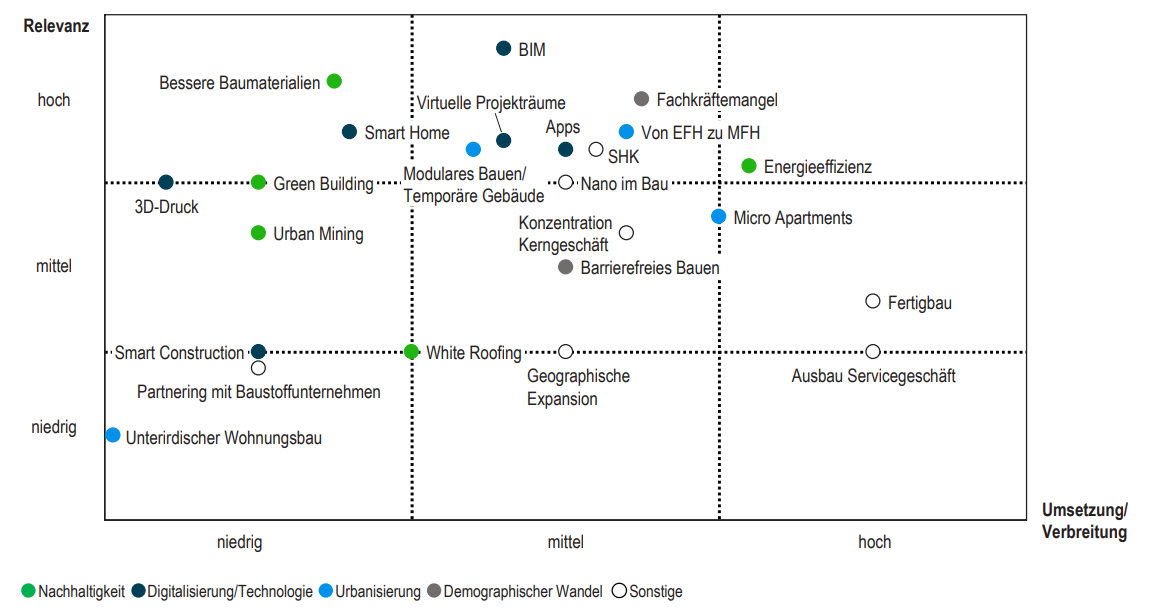
\includegraphics[scale=0.52]{bim-relevanz}
	\source{\citep[p.~20]{RolandBerger2016}}
	\caption{Megatrends Nachhaltigkeit und Digitalisierung in der Bauwirtschaft.}
	\label{fig:bim}
\end{figure}

\section{Motivation}
\label{c:intro:motivation}

Ziel der \glqq ORCA Software GmbH\grqq{} ist es, \ac{bim} noch mehr in die ORCA AVA zu integrieren. \ac{bim} bedeutet, dass die Planung von Bauprojekten vollständig auf digitaler Basis durchgeführt wird.  Für jeden Projektbeteiligten besteht somit jederzeit Zugriff auf alle projektrelevanten Daten wie Kosten, Mengen und Zeitabläufen. Somit können Baukosten einfacher ermittelt und der Bauprozess besser überwacht werden. In \autoref{fig:bim} ist zu sehen, dass \ac{bim} ein relevanter Begriff in der Baubranche ist. Die Verwendung in der Praxis ist allerdings noch nicht weit verbreitet. \citep[vgl.][p.~20]{RolandBerger2016} Mit dem \glqq \ac{ifc} First\grqq{} Ansatz ist das langfristige Ziel der ORCA AVA, das Thema \ac{bim} noch mehr abzudecken. Aus den Daten eines 3D-Gebäudemodells soll automatisch ein Ausschreibungstext generiert werden können. Wenn ein \ac{ifc}-Bauteile demnach schon alle Informationen beinhalten, soll damit eine Position mit Kurztext, Langtext, Menge, Preis und vordefinierten Kostengliederungen in den Programmteil Bauelemente der ORCA AVA übernommen werden können. Der erste Teil davon ist die Übernahme der Baumaterialien aus einer \ac{ifc}-Datei. Diese bietet die erste Kostengliederung für den \glqq \ac{ifc} First\grqq{} Ansatz. Die Übernahme von weiteren Daten aus dem \ac{ifc}-Modell können darauf aufgebaut werden. Aufgrund der hohen Relevanz des Themas, spricht das Ganze viele Kunden an und stellt somit ein effektives Werbemittel für den Verkauf der Software dar. 

Ein weiterer Trendbegriff, der mit der Programmerweiterung abgedeckt werden soll, ist \glqq Künstliche Intelligenz\grqq{} und \glqq Maschinelles Lernen\grqq{}. Das Suchinteresse der beiden Themen ist in \autoref{fig:ki-ml-trend} zu sehen. Die Werte geben das Google-Suchinteresse relativ zum höchsten Punkt im angegebenen Zeitraum an. Der Begriff \glqq Maschinelles Lernen\grqq{} hat seit Anfang 2015 ein steigendes Suchinteresse. Bei \glqq Künstliche Intelligenz\grqq{} ist das Suchinteresse von Anfang 2017 bis Ende 2021 konstant hoch. Der starke Anstieg ab November 2022 ist signifikant und korreliert wahrscheinlich mit der Veröffentlichung des Chatbots ChatGPT, wodurch auch Menschen außerhalb der Informatik erreicht wurden. Man erkennt insgesamt, dass das Interesse über die letzten Jahre stetig ansteigt. Die Abdeckung dieser Begriffe ist seit geraumer Zeit ein Wunsch der Vertriebsseite für den noch besseren Verkauf der Software. Die neue Programmerweiterung wäre der erste Einsatz von maschinellem Lernen. Es ist also zusätzlich auch ein Pilotprojekt in der ORCA AVA Entwicklung, um sich mit Machine-Learning-Algorithmen vertraut zu machen und Erfahrungen in diesem Themengebiet zu sammeln. 

Durch die genannten Punkte ist die Programmerweiterung dem Kano-Modell nach als Begeisterungsfeature zuzuordnen. Die Kundenzufriedenheit steigt also exponentiell mit dem Erfüllungsgrad der Anforderung. (siehe \autoref{fig:kano-model}) Mit der Zeit wandelt sich es dann erst in ein Leistungsfeature und irgendwann in ein Basisfeature. \citep[vgl.][p.~3-4]{Hölzing_2008} Es besteht also die Motivation die Erweiterung möglichst exklusiv zur Verfügung zu stellen. Es eignet sich somit sehr für die ORCA AVA \ac{ee} Edition.

\begin{figure}[h]
	\centering
	
	\begin{subfigure}{0.99\textwidth}
		\centering
	\includegraphics[width=1\textwidth]{künstiliche-intilligenz-trend}
		\caption{Suchinteresse: Künstliche Intelligenz}
		\label{FIG:ki-trend}
	\end{subfigure}
	\hspace{1cm}
	\begin{subfigure}{0.99\textwidth}
		\centering
	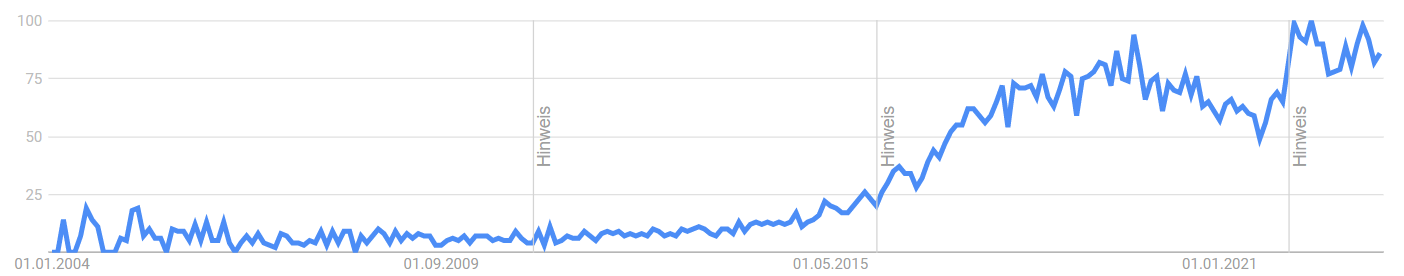
\includegraphics[width=1\textwidth]{machine-learning-trend}
		\caption{Suchinteresse: Machine Learning}
		\label{FIG:ml-trend}
	\end{subfigure}
	
	\caption[Google Suchinteresse von \glqq Künstliche Intelligenz\grqq{} und \glqq Maschinelles Lernen{}]{Google Suchinteresse der Begriffe \glqq Künstliche Intelligenz\grqq{} und \glqq Maschinelles Lernen\grqq{} von 2004 bis 2023}
	\label{fig:ki-ml-trend}
\end{figure}

\begin{figure}[h]
	\centering
	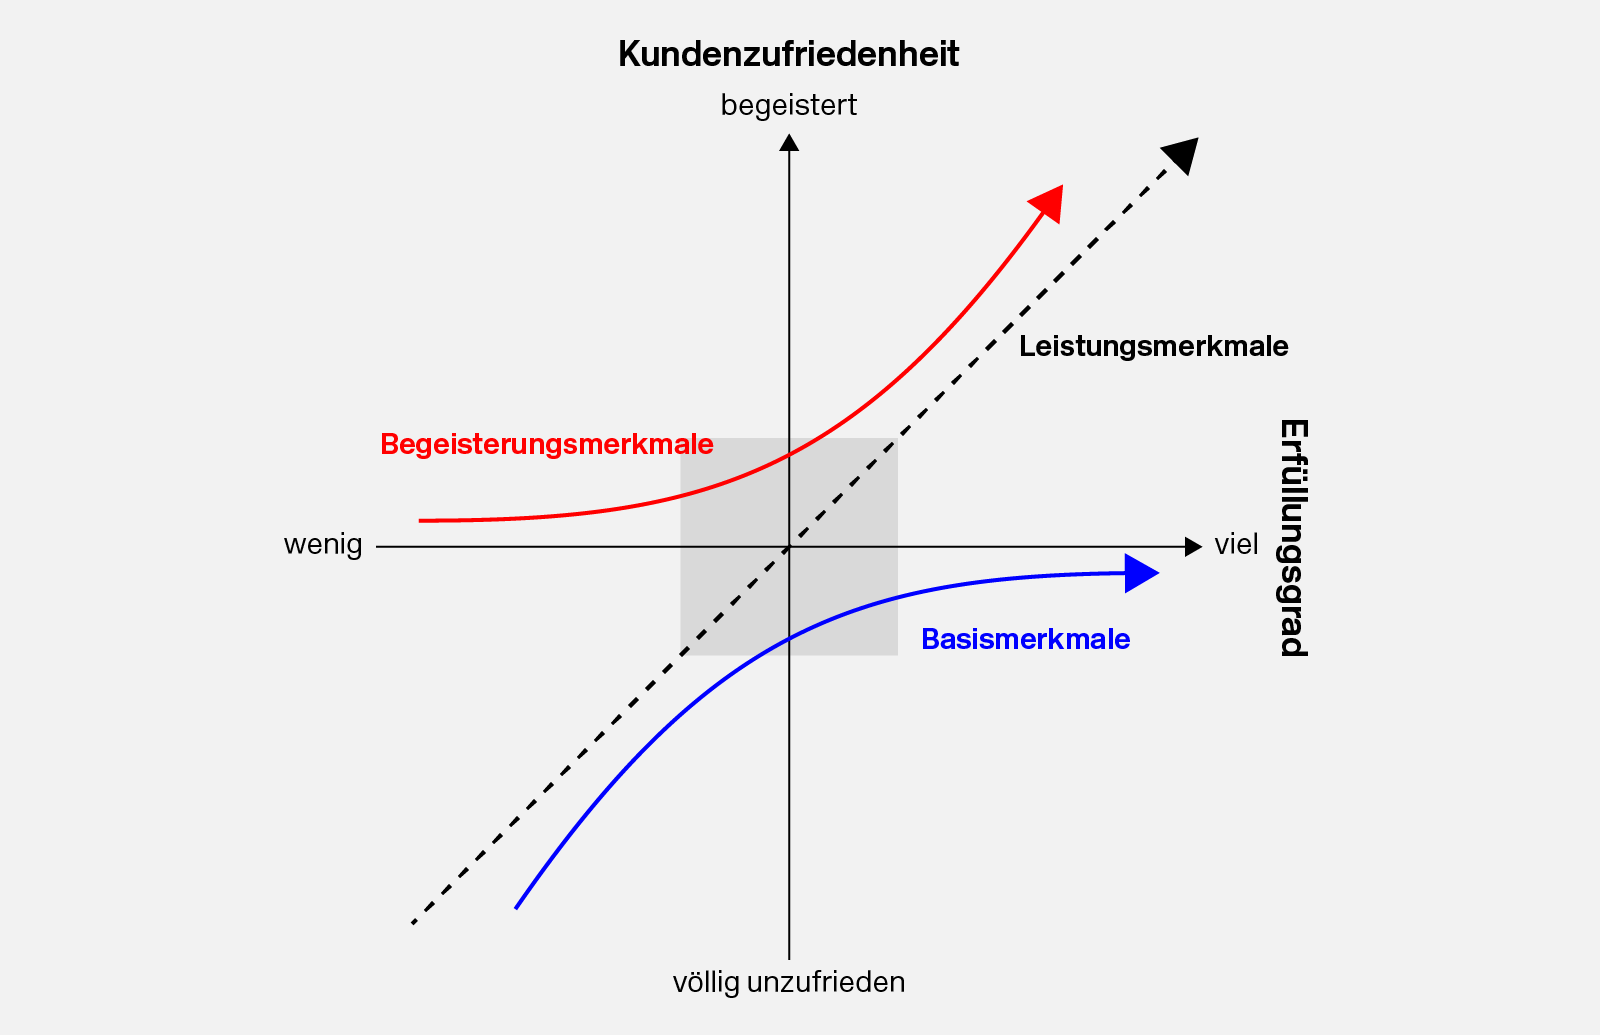
\includegraphics[width=\textwidth]{kano-modell}
	\source{https://dmexco-lightsails-media.s3.eu-central-1.amazonaws.com/wp-content/uploads/2021/01/04112832/Kano-Modell.png (Accessed: 2023-2-24) }
	\caption{Kano Modell der Kundenzufriedenheit}
	\label{fig:kano-model}
\end{figure}

\section{Ziel der Arbeit}
\label{c:intro:target}
Die Erstellung der Materialkostengliederung hängt hauptsächlich von den genutzten Algorithmen ab, welche die Materialien strukturieren. In dieser Arbeit soll neben dem Konzept für die Programmerweiterung, demnach vor allem der Algorithmus für die Strukturierung der Materialien erarbeitet werden. 
Um die Anforderungen aus \autoref{c:requirements:requirements} umsetzten zu können, muss dafür zuvor ein Ziel formuliert werden. Die Zieldefinition für diese Arbeit wird nach der SMART Technik definiert. Dabei muss ein Ziel folgende Eigenschaften haben:

\begin{itemize}
	\setlength\itemsep{0.01em}
	\item Spezifisch
	\item Messbar
	\item Attraktiv
	\item Realisierbar
	\item Terminiert
\end{itemize}

Anhand dieser Kriterien wurde folgendes Ziel definiert:


\goalshaded{Bis zum 15.06.2023 werden für die Implementierung passende Algorithmen nach den Kriterien der Messbarkeit (siehe \autoref{c:requirements:requirements:functional}) ausgewählt. Dazu wird ein \glqq Draftprojekt\grqq{} mit allen vollständigen funktionalen Anforderungen für die ORCA AVA implementiert. Zusätzlich sollen die Maßnahmen zur Qualitätssicherung (\autoref{c:qs}) durchgeführt werden.}

\section{Wissenschaftliche Vorgehensweise}
\label{c:intro:methodology:scientific_proceture}
Im Folgenden wird die wissenschaftliche Vorgehensweise der Arbeit aufgezeigt.
In \autoref{c:intro} wurde bereits die Ausgangssituation beschrieben, das Entwickeln der Programmerweiterung motiviert und des Ziel dieser Arbeit definiert. Im nächsten Kapitel, \autoref{c:basics}, werden Grundlagen erläutert, auf die diese Arbeit aufbaut. Im anschließenden \autoref{c:requirements} sollen die Problemstellung und Anforderungen analysiert werden. Danach (\autoref{c:conception}) wird eine Lösung für die Problemstellung theoretisch konzipiert und verschiedene mögliche Algorithmen erläutert und analysiert. Hierfür wird der Ablauf in die Textklassifizierung und die Feinstrukturierung aufgeteilt. In \autoref{c:comparison} werden die Algorithmen für diese beiden Schritte jeweils gegenübergestellt und nach den definierten Kriterien der Messbarkeit ausgewählt. \autoref{c:qs} zeigt die genutzten Maßnahmen der Qualitätssicherung auf. Am Ende wird das Ergebnis bewertet und ein Ausblick gegeben.


\chapter{Grundlagen}
\label{c:basics}
In diesem Kapitel werden die Grundlagen im Bereich der fachspezifischen Themen, Technik und Projektmanagement vermittelt. Das soll Verständnis für die folgenden Kapitel schaffen. Zuerst geht es um das Projektmanagement. Anschließend geht es um das Format \ac{ifc}, dessen Geschichte und dessen Nutzungsmöglichkeiten für diese Arbeit. Außerdem wird die Struktur und der Nutzen einer Kostengliederung in der ORCA AVA veranschaulicht.

\section{Projektmanagement}
\label{c:basics:project-management}
Bevor auf technische und fachliche Aspekte von \ac{ifc} und Kostengliederungen eingegangen wird, folgt die Einführung in das Projektmanagements mit SCRUM und \ac{devops}.

\subsection{Vorgehensmodell}
\label{c:basics:project-management:procedure_model}
Das Projekt wurde mithilfe agiler Softwareentwicklung durchgeführt. Im ORCA AVA Entwicklungsteam wird das SCRUM Modell verwendet. Die Entwicklung der Produkterweiterung in dieser Arbeit läuft in diesem SCRUM-Prozess.

\begin{definition}[Scrum]
	\glqq Scrum is a lightweight framework that helps people, teams and organizations generate value through adaptive solutions for complex problems. \grqq{} \citep[vgl.][p.~3]{scrum_2020}
\end{definition}

SCRUM verwendet einen iterativen, inkrementellen Ansatz. So kann Sprint für Sprint aus gewonnenen Erfahrungen der Entwicklungsablauf optimiert werden. \citep[vgl.][]{scrum_2020} Product Owner in der ORCA AVA Entwicklung ist die \glqq ORCA Software GmbH\grqq{}, in Vertretung des Produktmanagement-Teams. Die Umsetzung der Sprint-Ziele wird von einer Person implementiert.

\subsection{DevOps}
\label{c:basics:project-management:devops}
Die Bezeichnung \ac{devops} vereint die beiden Praktiken \glqq Development\grqq{}(Entwicklung) und \glqq Operations\grqq{}(Vorgänge). Die traditionelle Trennung von Entwicklung und Softwarebetrieb führt oft zu
Interessenskonflikten. Entwickler wollen stetig die Software verbessern und der Betrieb will Änderungen vermeiden, um die Stabilität des Systems zu gewährleisten. Durch \ac{devops} entsteht ein Softwareentwicklungsprozess, den man durch Praktiken wie Continous Integration, Continous Delivery, Continous Deployment, automatisiertes Teste, Infrastructure-as-Code und automatische Veröffentlichungen beschleunigt. DevOps steht auch für eine Entwicklungskultur mit offener Zusammenarbeit, Kommunikation, Transparenz und Eingestehen von Fehlern, um Konflikte im Team zu vermeiden. \citep[vgl.][]{devops_2021} Im Entwicklungsteam der ORCA AVA wird diese Praktik umgesetzt. Die technischen Hilfsmittel, die für den DevOps Prozess verwendet werden, sind in \autoref{c:qs:technical_aids} beschrieben.

\section{\acf{ifc}}
\label{c:basics:ifc}
Die Daten für die Material-Kostengliederung werden aus einem digitalem Gebäudemodell entnommen. Der öffentliche internationale Standard (ISO 16739-1:2018) für Gebäudemodelle ist \ac{ifc}. \citep[vgl.][]{BuildingSMART_IFC4_doc} Dieser wird auch in der bestehenden ORCA AVA benutzt, um den Ausschreibungsprozess zu unterstützen. \ac{ifc} Dateien können geöffnet, das 3D-Modell angezeigt und Informationen über das Modell in die Hauptsoftware übernommen werden.

\subsection{Geschichte}
\label{c:basics:ifc:history}
\ac{ifc} ist die Hauptleistung der \textit{buildingSMART International Ltd.}. Die non-profit Organisation will mit der Spezifikation den BIM Prozess fördern und voranbringen. \citep[vgl.][]{BuildingSMART_IFC}
Angefangen hat die Organisation als der Verein \textit{Industrieallianz für Interoperabilität IAI e. V.} mit Sitz in Berlin. 1994 startete die Entwicklung an dem offenen Datenmodellstandard \ac{ifc}. Dieser sollte die Anforderungen der Industrie an Interoperabilität gerecht werden und eine gemeinsame Basis zum Austausch von Informationen durch verschiedenen Anwendungen schaffen. Im Zusammenhang mit \ac{bim} sollten Daten lesbar, editierbar für verschiedene Systeme durch den Bauprozess und kompletten Lebenszyklus eines Gebäudes geteilt werden. \citep[vgl.][]{Laakso2012-oi} Nach einigen Prototypen wurde 1999 \ac{ifc} 2.0 veröffentlicht. Diese wurde bis 2007 mit der Version 2.3.0.1 stetig verbessert. Die Version 2.3 wird auch in heutigen Projekten noch verwendet. 2013 wurde \ac{ifc}4 veröffentlicht, welche mit der Version 4.0.2.1 die aktuellste, offizielle \ac{ifc} Version ist. Das Format wird weiterhin stetig weiterentwickelt. Neue Versionen stehen schon vor einer Abstimmung der \ac{iso}. \citep[vgl.][]{BuildingSMART_history_2022} Es gibt folgendermaßen aktuell zwei offizielle Versionen. Beide werden in der Praxis benutzt und sind, wie in \autoref{c:basics:ifc:usage} beschrieben, mit der ORCA AVA kompatibel.


\subsection{Format}
\label{c:basics:ifc:format}
Das \ac{ifc} Format kodiert folgende Daten:
\begin{itemize}
	\item Identität, Semantik, Attribute und Relationen von Objekten
	\item Abstrakte Konzepte wie Performance oder Kosten
	\item Prozesse wie z.B.Installationen und Operationen
	\item Personen wie z.B. Eigentümer oder Lieferanten
\end{itemize}
Die Spezifikation kann also für das Bauen, Betreiben oder Nutzen eines Gebäudes genutzt werden. \ac{ifc} ist ein Implementierungs-Unabhängiges Datenmodell, welches in verschiedenen Umgebungen und elektronischen Formaten benutzt werden kann. Es kann beispielsweise in eine relationales Datenbankschema gegossen oder auch als Dateiformat implementiert werden. Das weitverbreiteste Format ist \ac{spf} \citep[vgl.][]{Laakso2012-oi,BuildingSMART_IFC}. \ac{spf} ist das kompakteste Format für den dateibasierten Import und Export von \ac{ifc}-Dateien. Die Dateiendung des Formates ist \glqq \textit{.ifc}\grqq{}. Des Weiteren kann \ac{ifc} als \ac{xml} oder ZIP Datei verwendet werden. \citep[vgl.][]{BuildingSMART_IFC}

\subsection{Verwendung}
\label{c:basics:ifc:usage}
\begin{displayquote}
	\glqq Today, \ac{ifc} is typically used to exchange information from one party to another for a specific business transaction.\grqq{} \citep{BuildingSMART_IFC}
\end{displayquote}
In der ORCA AVA wird \ac{ifc} für das Einlesen und Übernehmen von Maßen und Mengen in die Ausschreibung verwendet. Es vereinfacht den Prozess, die in der \ac{cad}-Software erstellten Daten einfach in die Leistungsverzeichnisse der ORCA AVA zu überführen.
Die ORCA AVA kann \ac{ifc}-Dateien einlesen. Im \ac{ifc} Manager wird das 3D-Modell dann angezeigt. In dem geöffneten Fenster gibt es einige fachliche Ansichten, die jegliche \ac{ifc}-Daten nochmal fachlich abstrahieren. In den Ansichten können zum Beispiel bestimmte Maße oder die Anzahl verschiedener Bauteile, die aus dem \ac{ifc}-Modell ermittelt werden, in die ORCA AVA übernommen werden. Auch alle definierten Eigenschaften eines Bauteils sind in der Eigenschaften-Ansicht sichtbar. Hier kann man auch die Materialbezeichnung des Bauteils finden, die im Modell hinterlegt ist. In \autoref{fig:ifc-manager} ist die Oberfläche des \ac{ifc} Managers zu sehen. Man sieht die Materialangabe rechts unten im Eigenschaftenfeld unter dem 3D-Modell.

Für das Arbeiten mit \ac{ifc}-Dateien wird die open-source Bibliothek \textit{xbim-toolkit} \citep{LockleyXbimEssentialslibrary2017} verwendet. Die .NET Bibliothek kann \ac{ifc}-Dateien lesen, schreiben und anzeigen. Außerdem unterstützt es bei der Berechnung von komplexer Geometrie, um die Modelldaten für Analysen nutzbar zu machen. Die Entwicklung der Bibliothek startete 2007 und läuft seit 2009 in Zusammenarbeit mit der Norhumbria Untiversity. Mittlerweile bildet es die Standards \ac{ifc2x3} und \ac{ifc4} zu 100\% ab. Zudem bietet es an, auch \ac{ifc2x3} Modelle über das \ac{ifc4} Interface anzuprogrammieren. Somit können mit einer Codebasis beide Formate abgebildet und unterstützt werden. \citep[vgl.][]{Xbim_ltd_history}


\subsection{Möglichkeiten für die Materialangabe eines Bauteils}
\label{c:basics:ifc:buildingmaterial}
In einem \ac{ifc}-Modell können Materialien auf unterschiedliche Weise einem Bauteil zugewiesen werden. Die Spezifikation bietet die Klasse \textit{IfcMaterial}. Diese bildet fachlich ein Material ab. Es hat die Attribute Name, Description und Category.\citep[vgl.][]{ifc_material} Eine Instanz von \textit{IfcMaterial} kann mit einem Element oder Elementtyp über die \textit{IfcRelAssociatesMaterial} verbunden werden. Diese Zuweisung kann über verschiedene Weisen stattfinden. In \autoref{fig:material-single} ist eine direkte Zuweisung über das \textit{IfcRefAssociatesMaterial} zu sehen. Hier hängt das \textit{IfcMaterial} direkt am Element. 
Bei einer Platte mit mehreren Schichten kann das \textit{IfcMaterial} auch wie in \autoref{fig:layer-set} zu sehen an einem \textit{IfcMaterialLayerSet} zugewiesen sein. Jede Schicht hat hier seine eigene Dicke und eigene Materialangabe. Ein Träger kann das \textit{IfcMaterial} über ein \textit{IfcMaterialProfileSet} abgebildet haben. (siehe \autoref{fig:profile-set}) Bei einer Tür können verschiedene Materialien des Rahmens und der Verglasung über das \textit{IfcMaterialConstituentSet} abgebildet werden. (siehe \autoref{fig:constituent-set}) \citep[vgl.][]{ifc_material_association} Zusätzlich gibt es noch ältere Möglichkeiten Materialangaben an ein Element zu binden. In \ac{ifc2x3} gibt es die Klasse \textit{IfcMaterialList} \citep[vgl.][]{Thomas2007_MaterialList}. Diese Möglichkeit ist deprecated, in der Praxis kommt das \ac{ifc2x3} Format noch regelmäßig vor. Die \textit{IfcMaterialList} muss also auch beachtet werden. Neben verschiedenen Verbindungen zu \textit{IfcMaterial} hat jedes Element bei \ac{ifc} auch verschiedene Property Sets. Property Sets sind Container, die Eigentschaften je nach ihrem Namensattribut enthalten. Einige Property Sets sind in der Spezifikation des \ac{ifc} Standards enthalten. Es können auch zusätzlich benutzerdefinierte Property Sets erfasst werden. Diese können auch Informationen über das Material eines Elements enthalten. \citep[vgl.][]{ifc_property_set} Das PropertySet \textit{Pset\_MaterialConcrete} weist darauf hin, dass es sich z.B um Beton handelt.

Die Qualität der Materialkostengliederung hängt somit am Ende maßgeblich von den Materialangaben in der \ac{ifc}-Datei ab. Wenn Materialspezifikationen fehlen, ist auch das Ergebnis der Materialstrukturierung fehlerhaft.

\begin{figure}[h]
	\centering
	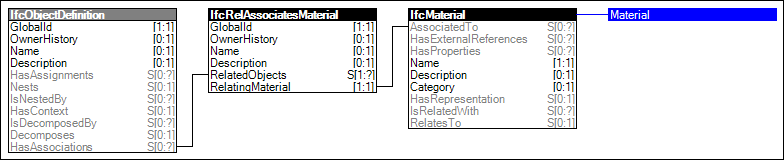
\includegraphics[width=\textwidth]{material-single}
	\source{\cite{ifc_material_graph}}
	\caption{\ac{ifc}: Material Single Association}
	\label{fig:material-single}
\end{figure}

\section{Das Format Kostengliederung in der ORCA AVA}
\label{c:basics:coststructure}
Die Kostengliederung bietet eine Struktur, um Gesamtkosten einer Baumaßnahme in Kostengruppen unterteilt auswerten zu können. Logisch zusammengehörende Kosten können so in eine \ac{kg} zusammengerechnet werden. Außerdem handelt es sich beim Aufbau um eine Baumstruktur, wodurch Kostengruppen hierarchisch addiert werden können. In \autoref{fig:cost-structure} ist ein Beispiel einer Kostengliederung mit Materialien zu sehen. Der Gliederungspunkt \textit{Mineralisch} wird in die Unterpunkte \textit{Mauerwerk}, \textit{Beton}, \textit{Dachziegel} und \textit{Kies} unterteilt. Um die Kosten aller Mineralien zu erfassen, können die Kosten der Unterpunkte für den Gliederungspunkt \textit{Mineralisch} addiert werden.
Bei einem Bauprojekt kann man so Kosten über alle Projektphasen vergleichen. Von der Kostenschätzung über die Ausschreibung bis zur Rechnungsfreigabe. So können Kostenauswertungen nach den verschiedenen Kostengruppen durchgeführt werden. In einem ORCA AVA Projekt kann man verschiedene Kostengliederungen definieren. Es existieren bereits Standardkostengliederungen beim Erstellen eines neuen Projektes. Zusätzlich können neue Kostengliederungen erstellt oder importiert werden.\citep[vgl.][]{helpdesk-kostengliederungen}

\chapter{Problemstellung und Anforderungen}
\label{c:requirements}
Im folgenden Kapitel werden die Problemstellung und Anforderungen aufgeführt, um das Projekt einzugrenzen. Diese kommen vom Auftraggeber, der \glqq ORCA Software GmbH\grqq{} selbst.

\section{Problemstellung}
\label{c:requirements:problem}

Die Problemstellung entsteht aus der Ausgangssituation (\autoref{c:intro:start}) und der Motivation (\autoref{c:intro:motivation}) der Bausoftware ORCA AVA. Der \ac{bim} Prozess soll noch mehr in die Software integriert werden. Deswegen wurde sich die Programmerweiterung der Materialkostengliederung gewünscht, um den ersten Schritt zu \glqq \ac{bim} First\grqq{} zu schaffen. Die Problemstellung dieser Arbeit bezieht sich der dementsprechenden Umsetzung dieser Programmerweiterung:

\begin{problem}
	\label{p:main}
	Wie lässt sich am besten eine Liste vom Materialbezeichnungen in eine hierarchische Material-Kostengliederung strukturieren?
\end{problem}

Da es sich hier um eine offene Frage handelt, sind Spielräume für die Antwort offen. Es soll ein Konzept und eine Architektur für die Programmerweiterung entstehen. Um ein fachlich richtiges Ergebnis der Strukturierung zu erreichen, ist aber vor allem folgende Problemstellung wichtig:

\begin{problem}
	\label{p:algorithm}
	Welcher \ac{nlp} Algorithmus eignet sich am besten für das Klassifizieren und Strukturieren von Material-Daten? 
\end{problem}

Bei dieser offenen Frage, soll am Ende ein Algorithmus oder eine Kombination aus einer Auswahl ausgewählt werden. Um verschiedene Ansätze und Algorithmen vergleichen zu können, benötigt man Kriterien der Messbarkeit. Diese werden in \autoref{c:conception:classification:criteria} und \autoref{c:conception:fine-structuring:criteria} definiert. So kann man neben der Berücksichtigung der Anforderungen den geeignetsten Algorithmus auswählen, um die Problemstellungen \ref{p:main} und \ref{p:algorithm} zu lösen.

%\begin{problem}
%	\label{p:different-files}
%	Wie verhält sich die Variabilität der Materialangabe in verschiedenen %\ac{ifc}-Dateien für den jeweiligen Kostengliederungs-Import?
%\end{problem}

\section{Anforderungen}
\label{c:requirements:requirements}
Alle definierten Anforderungen kommen vom Projektmanagement Team der ORCA Software GmbH und dem Teamleiter der ORCA AVA Entwicklung. Die Gesamtheit von Anforderungen kann in funktionale Anforderungen, Leistungsanforderungen, spezifische Qualitätsanforderungen und Randbedingungen unterteilt werden.\citep[vgl.][]{glinz_2007} Durch die beschriebenen Anforderungen aus diesem Abschnitt entstand das beschriebene Ziel der Arbeit (siehe \autoref{c:intro:target})

\subsection{Funktionale Anforderungen}
\label{c:requirements:requirements:functional}

\begin{definition}[Funktionale Anforderung]
	\label{def:functional-requirement}
	\glqq A functional requirement is a requirement	that pertains a functional concern.\grqq{}\citep{glinz_2007}
\end{definition}

Wie in \autoref{def:functional-requirement} beschrieben, geht es bei einer funktionalen Anforderung um die Funktion einer Software. Die im Mittelpunkt stehende Funktion ist die Erstellung der hierarchischen Materialstruktur (\autoref{r:main}). Nach dem Importieren der Materialstruktur aus einer \ac{ifc}-Datei soll bei der Übernahme von Mengen die Materialkostengliederung automatisch zugewiesen werden (\autoref{r:takeover}). Zusätzlich sollen die Ergebnisse von \autoref{r:main} sich stetig verbessern. Dafür soll eine Möglichkeit geschafft werden, dass Nutzer der ORCA AVA Verbesserungen eintragen können und sich somit den Trainingsdatenbestand erweitert und verbessert (\autoref{r:percistance}).

\begin{requirement}
	\label{r:main}
	Aus einer Liste von Materialbezeichnungen soll eine hierarchische Baumstruktur entstehen, welche in einer ORCA AVA Kostengliederung benutzt werden kann.
\end{requirement}

\begin{requirement}
	\label{r:takeover}
	Bei der Übernahme einer Menge aus dem \ac{ifc} Manager soll die passende Material-Kostengruppe zugewiesen werden.
\end{requirement}

\begin{requirement}
	\label{r:percistance}
	Bei einem falsch zugewiesenem Material in der generierten Kostengliederungsstruktur soll eine persistente, dauerhafte Verbesserung des Benutzers möglich sein.
\end{requirement}

Die funktionalen Anforderungen werden noch nicht direkt in die ORCA AVA integriert. Wie im Ziel der Arbeit erläutert, wird ein Draftprojekt zur Demonstration der Funktionen dienen. Somit kann zuerst überprüft werden, ob die gewünschte \autoref{r:main} fachlich gut genug ist, um sie in die Hauptsoftware zu integrieren. Ein Vorschlag zur Integration in die Oberfläche der ORCA AVA wird am Ende in \autoref{c:closing:outlook} gegeben.



\subsection{Weitere Anforderungen}
\label{c:requirements:requirements:additional}

Neben den funktionalen Anforderungen gibt es vor allem technische Anforderungen an die Programmerweiterung. Diese wurden vom Teamleiter der ORCA AVA Entwicklung gestellt:

\begin{requirement}
	\label{r:language}
	Die Programmerweiterung soll wenn möglich in .NET (C\#) implementiert werden. Darüber hinaus ist auch das Nutzen von Python möglich.
\end{requirement}

Die technische Einschränkung der \autoref{r:language} macht den Code und die Programmerweiterung für die ORCA Software GmbH wartbar. C\# ist die Hauptsprache der Firma. Durch das dementsprechende Wissen in der Entwicklung, kann bei Fehlerbehebungen eine erneute Einarbeitungszeit vermeidet werden. Zusätzlich gibt es auch schon ein Modul für \acf{ade}, das Pythoncode verwendet.

\begin{requirement}
	\label{r:improvement}
	Die Materialstrukturierung soll mit der Erweiterung der Datengrundlage immer besser gemacht werden können.
\end{requirement}

Durch das Einlesen neuer \ac{ifc}-Dateien von Benutzern, werden immer neue unklassifizierte Materialbezeichnungen gesammelt, die die Datengrundlage erweitern. Somit müssen neue Begriffe klassifiziert werden können, um das Modell stetig zu verbessern. Dementsprechend müssen \ac{ki}-Modelle auch immer wieder neu trainierbar sein. ORCA Internen Mitarbeiter sollen also eine Möglichkeit zum Klassifizieren der Daten zur Verfügung stehen haben.

\chapter{Theoretische Konzeption}
\label{c:conception}
In diesem Kapitel wird ein theoretisches Konzept für das Lösen der Problemstellung erstellt und begründet. Zuerst wird das allgemeine Konzept vorgestellt. Dann werden mögliche Algorithmen erläutert und evaluiert, wie sie zu den Anforderungen passen. Im Folgekapitel werden die Algorithmen miteinander verglichen und der geeignetste ausgewählt.

\section{Grundlegende Architektur und Vorgehensweise}
\label{c:conception:architecture}
In diesem Abschnitt wird das erarbeitete Konzept für die Erweiterung vorgestellt und begründet. In \autoref{fig:usecasediagramm} ist ein Anwendungsfalldiagramm der neuen Funktionen zu sehen. Die Anwendungsfälle des Benutzers der ORCA AVA decken sich mit den schon beschriebenen funktionalen Anforderungen in \autoref{c:requirements:requirements:functional}. In \autoref{fig:func-import}, \ref{fig:func-takeover} und \ref{fig:func-rating} sind Flussdiagramme für diese drei Anwendungsfälle zu sehen. Die zusätzlichen Anwendungsfälle der AVA Entwickler ergeben sich aus \autoref{r:improvement}.

\begin{figure}[h]
	\centering
	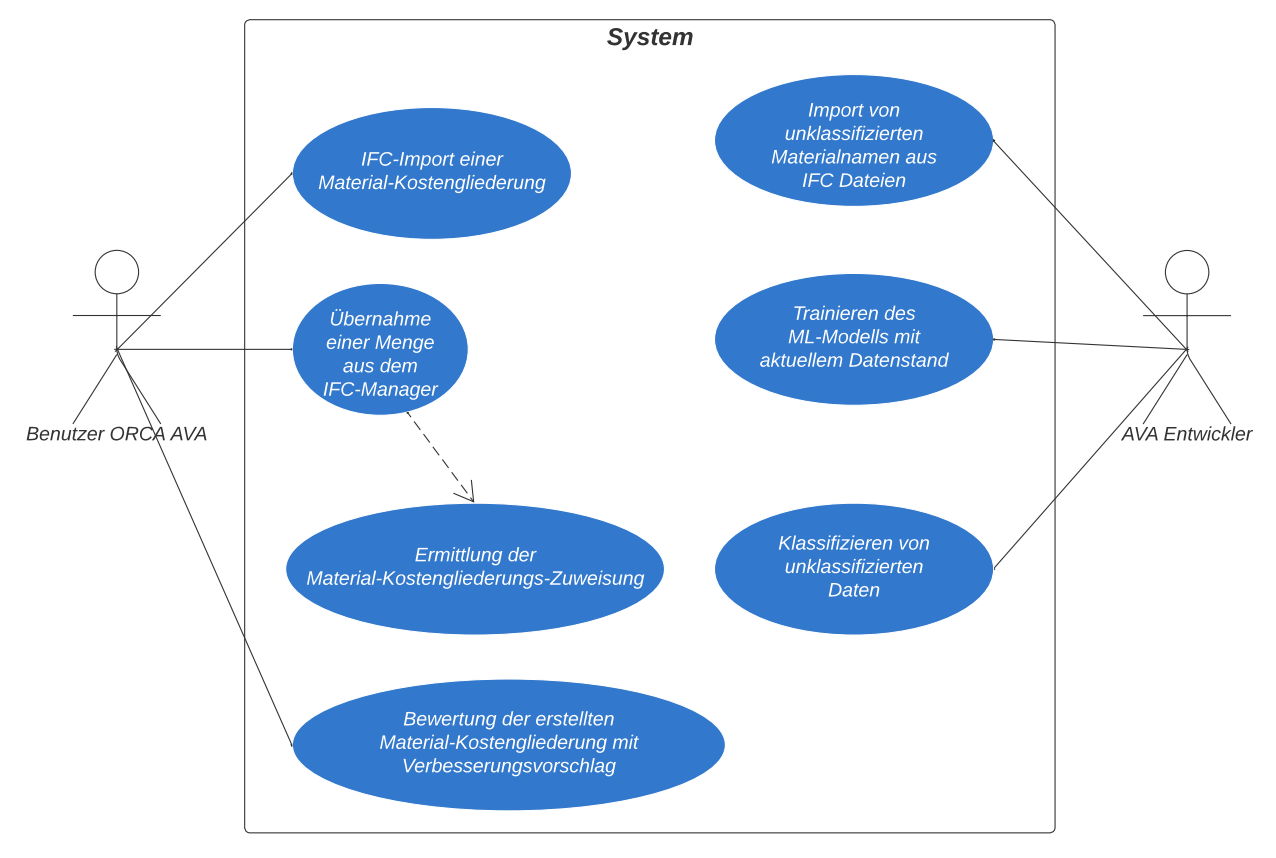
\includegraphics[width=\textwidth]{anwendungsfalldiagramm}
	\caption{Anwendungsfalldiagramm}
	\label{fig:usecasediagramm}
\end{figure}

Das Ergebnis des Hauptanwendungsfalles der Materialstrukturierung ist abhängig von den Inhalten der \ac{ifc}-Datei. Durch die Nutzung verschiedener \ac{cad}-Programme und eigene Vorlieben bei der Materialangabe der ORCA AVA Benutzer entstehen viele unterschiedliche Inhalte bei der Materialangabe. Um diese komplexe Problemstellung zu vereinfachen, werden Materialien zuerst nach dem \glqq Teile-und-hersche\grqq{} Verfahren in Oberkategorien klassifiziert. In \autoref{fig:material-categories} sind die Oberkategorien mit Beispielen aufgelistet. So müssen anschließend nur noch eine kleinere Liste von Materialien einer Oberkategorie jeweils weiter hierarchisch strukturiert werden.

In \autoref{fig:distribution-diagramm} ist ein Verteilungsdiagramm mit allen relevanten Objekten zu sehen. Auf dem lokalem Computer des Benutzers laufen die beiden Prozesse der ORCA AVA und des \ac{ifc} Managers. Die ORCA AVA kommuniziert mit einem Webserver über \ac{rest}. Dieser verwaltet die anhängende \ac{sql} Datenbank und übernimmt das Ausführen der funktionalen Anforderungen.

\subsection{Implementierung als Web-Service}
\label{c:conception:architecture:service}
Für die Materialstrukturierung ist ein neuer Webservice vorgesehen, mit dem die ORCA AVA kommunizieren kann. Dies bietet einige Vorteile:

\begin{itemize}
	\setlength\itemsep{0.3em}
	\item Der Import greift immer auf das aktuellste \ac{ki}-Modell zu, welches zentral verwaltet werden kann
	\item Wegen der nötigen Verwendung von Python muss nicht bei jedem Client eine lauffähige Pythonumgebung vorhanden sein oder durch das Setup installiert werden.
	\item Neue Materialbezeichnungen und Klassifizierungen werden direkt zentral in der Datenbank persistiert.
	\item Eine Änderung/Verbesserung der Datengrundlage kann durch automatisches Trainieren direkt zu einem verbessertem \ac{ki}-Modell für alle Nutzer führen.
\end{itemize}

Für die ORCA AVA bestehen schon Services für die Bereitstellung von News, die Lizenzierung oder das Updaten der Software. Durch die Vorgabe der ORCA Software GmbH wird der Service mit dem Framework ASP.NET implementiert. ASP.NET ist ein Open-Source und Plattform-unabhängiges Web-Framework für die Entwicklung cloudbasierter Anwendungen wie Web-Applikationen, \ac{iot}-Apps oder mobile Backends. \citep[vgl.][]{asp-net}. Die Architektur dieses Services entspricht dementsprechend den schon existierenden Services.

Daten werden über den Service in einem \ac{sql}-Datenbankserver gespeichert. Hier werden auch die ORCA Software GmbH internen Standards verwendet. Daten für den Material-Kostengliederungs-Import sind in der Tabelle \textit{Materials} persistiert. Die Tabellendokumentation ist in \autoref{fig:db-scheme} zu sehen. Zusätzlich bestehen Tabellen für die Autorisierung der Zugriffe auf den Service.

\begin{figure}[h]
	\centering
	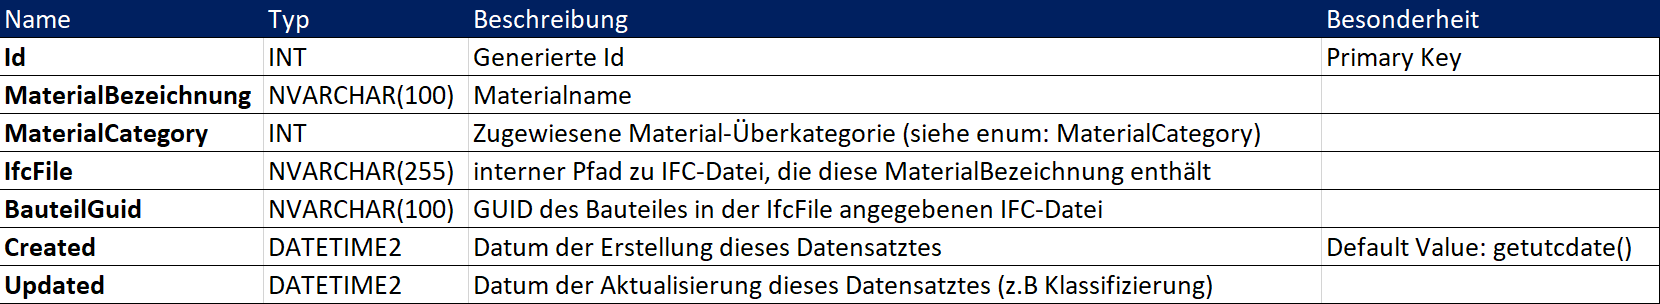
\includegraphics[width=\textwidth]{db-scheme}
	\caption{Dokumentation der Datenbanktabelle \textit{Materials}}
	\label{fig:db-scheme}
\end{figure}

\subsection{Konzept der Materialstrukturierung}
\label{c:conception:architecture:structuring}
Der Ablauf der Materialstrukturierung ist in drei Schritten aufgeteilt. Materialien werden nach dem Einlesen zuerst nach dem Preprocessing in übergeordnete Kategorien klassifiziert. Danach wird jede Überkategorie nochmals feiner strukturiert.
Dieser Ablauf ist in \autoref{fig:structurize-process} anhand eines Beispiels zu sehen. Am Ende entsteht bei erfolgreicher Feinstrukturierung eine Baumstruktur mit einer Tiefe von drei. Falls nach der Zuweisung in die Überkategorien mehr als 2 Materialien in der gleichen Kategorie sind, wird weiter fein-strukturiert.

\begin{figure}[h]
	\centering
	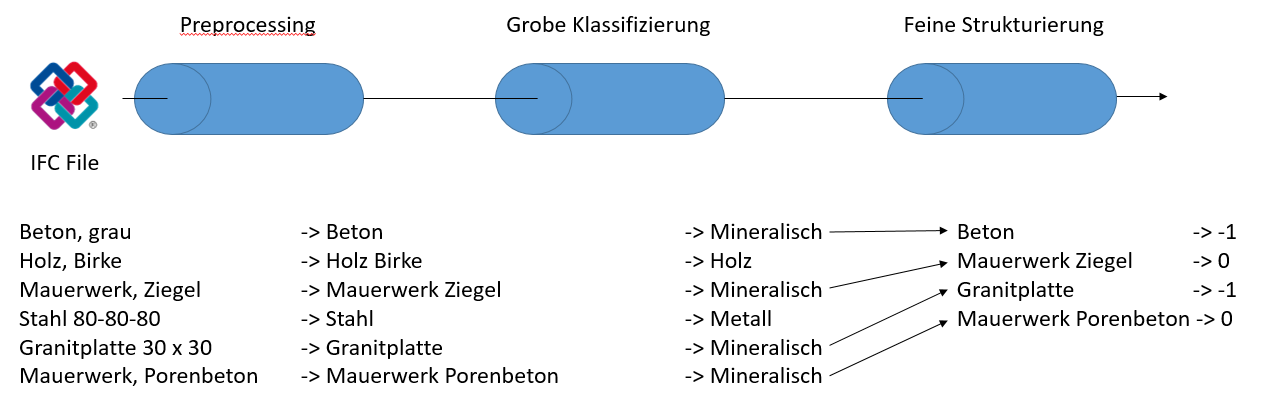
\includegraphics[width=\textwidth]{structurize-process}
	\caption{Ablauf der Strukturierung mit Beispiel}
	\label{fig:structurize-process}
\end{figure}

Bei der Strukturierung von Materialien gibt es einige \ac{nlp} spezifische Probleme, die gelöst werden müssen. 
\begin{problem}
	\label{p:shorttext}
	Bei den Materialangaben handelt es sich um sehr kurze Stichpunkte aus nur einem oder wenigen Wörtern. (z. B. Metall, Edelstahl - gebürstet)
\end{problem}

\autoref{p:shorttext} ist ein bekanntes, aber noch wenig erforschtes Problem in der Textklassifizierung. Textklassifizierungen stützen sich meistens auf Textrepräsentationen. Diese machen den Text durch Vektorisieren für den Klassifizierungsalgorithmus erst lesbar. Bei der Repräsentation von Texten haben kurze Texte folgende Nachteile:

\begin{itemize}
	\setlength\itemsep{0.1em}
	\item Kurzen Texten fehlt es an Kontext. Kontextbezogene Worteinbettungen wie z.B. Word2Vec führen folgendermaßen zu unbrauchbaren Textrepräsentationen für die Textklassifizierung.
	\item Kurze Texte entsprechen nicht immer der Syntax der natürlichen Sprache
	\item Kurze Texte sind in der Regel mehrdeutig, weil sie
	Polyseme und Tippfehler enthalten. \citep[vgl.][]{ijcai2017p406}
\end{itemize}

Um das Problem zu überwinden, schlagen \cite{ijcai2017p406} und \cite{chen2019deep} vor, mehr Syntax und Semantik aus den kurzen Texten zu erfassen, in dem man, mithilfe einer bekannten Wissensbasis, die Texte mit Merkmalen anreichert. Die Informationen aus dem Text alleine, reichen nicht aus, um die Bedeutung des Textes in einer Textrepräsentation gut darzustellen.
\cite{Qingyuan2019} nutzt unter anderem Wikipedia2Vec, um mit diesem Modell eine Textrepräsentation der Kurztexte zu ermitteln. Durch den mitgegebenen Kontext über das Wikipedia2Vec Modell wird so dem Wort seine Bedeutung der Textklassifizierung mitgegeben.

\begin{problem}
	\label{p:technical-term}
	In den Materialangaben kommen viele Fachbegriffe aus der Baubranche vor.
\end{problem}
Ein weiteres Problem ist \autoref{p:technical-term}. Laut \cite{nooralahzadeh2018evaluation} gibt es viele vortrainierte Worteinbettungs-Modelle, die sich aber auf den allgemeinen Bereich der Sprache fokussieren. Diese können Fachbegriffe oft schlecht verarbeiten, da die zum Trainieren genutzten Texte, diese Wörter nicht beinhalten.

Wie diese Probleme gelöst beziehungsweise umgangen werden, wird in den jeweiligen Abschnitten der verschiedenen analysierten Algorithmen in  \autoref{c:conception:classification} und \autoref{c:conception:fine-structuring} erläutert.

\subsection{Konzept für das Auslesen von Materialien aus einer \ac{ifc} Datei}
\label{c:conception:architecture:ifc-material-extraction}
Bevor jegliche Klassifizierung und Strukturierung stattfinden kann, müssen die Materialien erst aus der \ac{ifc}-Datei extrahiert werden. In \autoref{c:basics:ifc:buildingmaterial} wurden bereits die theoretischen Möglichkeiten der Materialangabe in der \ac{ifc}-Spezifikation aufgezählt.

Über schon vorhandenen Abstraktion des \textit{xbim-toolkit} (siehe \autoref{c:basics:ifc:usage}) kann eine \ac{ifc}-Datei eingelesen werden. Über das instanziierte Objekt \code{IfcProject} kann dann auf alle Daten der Datei zugegriffen werden. Hier wird ein neuer \code{MaterialsManager} als Attribut des \code{IfcProject} hinzugefügt. Über die Methode \code{Enumerable<Material> GetMergedMaterials()} im \code{MaterialsManager} können alle Materialangaben aus einer \ac{ifc}-Datei ausgelesen werden. Die Methode iteriert über jeden bekannten Materiallink mit seinem jeweiligen Objekt, teilt diese Links nach ihrem jeweiligen Materialtyp (z. B. LayerSet) auf und liest die Materialbezeichnungen entsprechend dem Materialtypen aus. Am Ende liefert die Methode also alle Materialbezeichnungen in einer List mit der jeweiligen \ac{guid} des Bauteiles.
Das Extrahieren der Materialien passiert clientseitig in der ORCA AVA. So muss dem Service nicht eine ganze Datei, sondern lediglich die Liste der Material-Zeichenketten übergeben werden. Zusätzlich spart man sich die Zeit des Einlesens der \ac{ifc}-Datei, wenn diese schon im \ac{ifc}-Manager geöffnet ist.

\subsection{Preprocessing der Materialien}
\label{c:conception:architecture:preprocessing}
Nach dem Einlesen beginnt das Preprocessing der Materialien.
Das Preprocessing ist ein wichtiger Schritt vor einer Klassifizierung. Es hat Auswirkungen auf die Genauigkeit, Interpretierbarkeit und Robustheit des Gesamtalgorithmus aus. \citep[vgl.][]{Zelaya_2019} Materialbezeichnungen aus \ac{ifc}-Dateien können verrauscht und uneinheitlich sein, da es sich um ein Freitextfeld handelt. Die Vorverarbeitung der Daten hilft, die Daten zu säubern und auf das wesentliche reduzieren. \citep[vgl.][]{Priyanga_2016}
Die Vorverarbeitungsstufe besteht normalerweise aus Aufgaben wie Tokenisierung, Entfernung von Stoppwörtern, Umwandlung in Kleinbuchstaben und Stemming. \citep[vgl.][]{Uysal_2014}
Für die Materialstrukturierung wird das Preprocessing als erster Schritt aus der Textklassifizierung extrahiert. Somit wirkt sich das Preprocessing auf beide weiteren Schritte (Textklassifizierung und Feinstrukturierung) aus. Außerdem wird das Preprocessing zusätzlich für die Zuweisung der Materialkostengliederung bei der Mengenübernahme als erster Schritt gebraucht.
Konkret wird beim Preprocessing folgende Schritte durchgeführt. Als Erstes werden alle Sonderzeichen bis auf \glqq /\grqq{} entfernt. Oft befinden sich in der Bezeichnung auch Größen- und Farbangaben, welche irrelevant für die Materialbeschaffenheit sind.
Mithilfe von Regex werden Farben, RGB-Farbcodes (z. B. \textit{60 - 60 - 60}) und Größenangaben (z. B. \textit{400 x 300}) herausgefiltert. Anschließend wird der Text in Worttokens, jeder Token in Kleinbuchstaben umgewandelt und unnötige Leerzeichen entfernt. Aus \textit{\glqq Kunststoff - grau 80-80-80\grqq{}} wird z. B. \textit{\glqq 'kunststoff'\grqq{}} und aus \textit{\glqq Beton- C30/37 Verputzt\grqq{}} wird \textit{\glqq 'beton', 'c30/37', 'verputzt'\grqq{}}

\section{Algorithmen für die Textklassifizierung}
\label{c:conception:classification}
Die Textklassifizierung ist nach dem Preprocessing der zweite Schritt der Materialstrukturierung. Hier werden die Materialien, den in \autoref{fig:material-categories} aufgelisteten Überkategorien, zugeordnet.
Technisch wird dieser Schritt mit der .NET-Bibliothek \textit{ML.NET} \citep[vgl.][]{Ahmed_2019} implementiert. Das Nuget-Package ist für die Erstellung benutzerdefinierte Modell für maschinelles Lernen. \citep[vgl.][]{mlnet_doc2022} Da die Bibliothek die Anforderungen für die Textklassifizierung gut erfüllen kann, kann die technische \autoref{r:language} für diesen Schritt eingehalten werden. Die Bibliothek kann direkt in den ASP.NET-Service integriert werden.
In diesem Kapitel wird zuerst der Ablauf einer normalen Textklassifizierung erläutert, die Kriterien der Messbarkeit festgelegt und dann die verschiedenen Algorithmen von \textit{ML.NET} analysiert.

\subsection{Ablauf einer Textklassifizierung}
\label{c:conception:classification:steps}
Die Stufen bei der Klassifikation von Texten sind in \autoref{fig:classification:flow} zu sehen. Alle diese Stufen wirken sich auf das Ergebnis der Klassifizierung aus:

\begin{figure}[h]
	\centering
	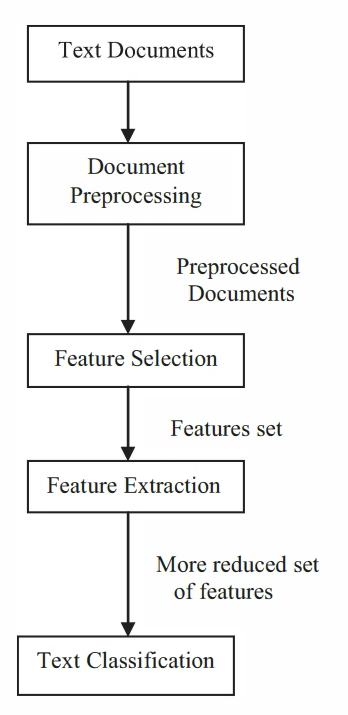
\includegraphics[width=0.3\textwidth]{classification-flow}
	\source{\cite{Foram_2016}}
	\caption{Stufen der Textklassifizierung}
	\label{fig:classification:flow}
\end{figure}

\subsubsection{Preprocessing}
Das in \autoref{c:conception:architecture:preprocessing} beschriebene Preprocessing findet als erster Schritt der ganzen Materialstrukturierung statt. Ein zusätzliches Preprocessing für die Textklassifizierung gibt es nicht.

\subsubsection{Feature Selection}
Beim Schritt der Feature Selection werden irrelevante Informationen für die Klassifizierung aus den Ausgangsdaten entfernt. Da es bei der Materialstrukturierung nur die Materialbezeichnung als Feature gibt, muss keine Auswahl aus einem Feature-Set getroffen werden. Es werden lediglich Größen- und Farbangaben aus dem Material-String im Preprocessing entfernt.

\subsubsection{Feature Extraction}
\begin{definition}[Feature extraction]
	\label{def:feature-extraction}
	\glqq Feature extraction addresses the problem of finding the most compact and informative set of features, to improve the efficiency or data storage and processing.\grqq{} \citep{Guyon2006}
\end{definition}
Bei der Feature Extraction geht es darum, die rohen Daten in eine numerische Darstellung zu bringen, die möglichst kompakt ist, ohne aber relevanten Informationen zu verlieren.
Auch die im Preprocessing entstandenen Worttokens sind noch Zeichenketten, die in eine numerische Darstellung umgewandelt werden müssen.

\subsubsection{Classification stages}
Nachdem die vorherigen Schritte auf die Daten ausgeführt wurde, kann das Training für die Klassifizierung durchgeführt werden.

\subsection{Kriterien der Messbarkeit}
\label{c:conception:classification:criteria}
Für die Textklassifizierung sind folgende Kriterien der Messbarkeit wichtig:

\subsubsection{Genauigkeit}
Die Genauigkeit bei maschinellem Lernen misst die Wirksamkeit eines Modells. Klassifizierte Daten werden in einen Testdatensatz und einen Trainingsdatensatz geteilt. Mit dem Testdatensatz wird das trainierte Modell getestet. Das Ergebnis der Genauigkeit stellt eine prozentuale Angabe der Übereinstimmung des Testdatensatzes zum trainierten Modell dar. \citep[vgl.][]{select_ml_2021}

\subsubsection{Interpretierbarkeit}
\begin{definition}[Interpretierbarkeit]
	\label{def:interpretability}
	\glqq Interpretability is the degree to which a human can understand the cause of a decision.\grqq{}\citep{miller_2017}
\end{definition}
Hier geht es darum, die Ergebnisse des Algorithmus nachzuvollziehen zu können. Alleine die Genauigkeit reicht nicht dazu aus, einem Machine-Learning-Algorithmus vertrauen zu können.
Ein Modell ist besser interpretierbar als ein anderes Modell, wenn seine Entscheidungen für einen Menschen leichter nachvollziehbar sind als die Entscheidungen des anderen Modells. Die Interpretierbarkeit kann man nicht direkt messen. Sie entsteht aus der Erfahrung über den Algorithmus und die Nachvollziehbarkeit der vorhergesagten Ergebnisse durch Testen.  \citep[vgl.][]{molnar2022} Das Endergebnis der Textklassifizierung aus verschiedenen \ac{ifc}-Dateien, wird fachlich vom Produktmanagement bewertet, da diese das fachliche Wissen haben, um das Ergebnis bewerten zu können. Die Robustheit ist somit auch sehr vom Preprocessing abhängig.

\subsubsection{Robustheit}

Von Deep-Learning-Algorithmen erwartet man, dass sie robust gegen kleine Störungen in der Eingabe sind. Es wurde allerdings schon festgestellt, dass kleine Störungen teilweise das Ergebnis ändern können. \citep[vgl.][]{Szegedy_2013} Dies kann auch bei anderen Machine Learning Algorithmen auftreten. In Bezug auf die Materialeingabe sollen zum Beispiel verschiedene Satzzeichen keinen Einfluss auf das Ergebnis haben. Die Materialbezeichnung \glqq Holz, Birke\grqq{} und \glqq Holz - Birke\grqq{} sollen mit dem Algorithmus auf das gleiche Ergebnis führen.

\subsubsection{Performance}

Aspekte wie Geschwindigkeit und Ressourcenbedarf spielen eine sekundäre Rolle. Wenn es den Anwendungsfluss allerdings sehr beeinträchtigt und verlangsamt, scheidet er als Option aus. Zum Punkt Performance zählt auch die Trainingsdauer des Algorithmus. Diese kann beim Verglich von verschiedenen Algorithmen helfen.\\

Konkret für die Textklassifizierung gilt als Kriterien der Messbarkeit die Genauigkeit, und sekundär die Ausführungsgeschwindigkeit und Trainingsdauer. Der Trainingsdatensatz wird aufgeteilt. 80 \% werden für das Trainieren und 20 \% für die Evaluation genutzt. Die benötigten Werte werden von \textit{ML.NET} geliefert und können für die Auswertung verwendet werden. Bei der Genauigkeit ist vor allem die \textit{MicroAccuracy} entscheidend, da sie den Durchschnitt der Datensätze über alle Klassen hinweg berechnet. Aufgrund des Klassenungleichgewichts gibt die \textit{MacroAccuracy} eine leicht verzerrte Genauigkeit zurück, dass sie nur die durchschnittliche Genauigkeit der einzelnen Klassen berechnet. Für die Genauigkeit wird auch der \textit{LogLoss} in Betracht gezogen. Zusätzlich wird eine Konfusionsmatrix erstellt, welche die Anzahl der vorhergesagten Klassen im Vergleich zu den tatsächlichen Klassen wiedergibt. \citep[vgl.][]{metrics_doc}
Die Trainingsdauer wird mithilfe der \code{Stopwatch}-Klasse im Code gemessen. Der Service wird dabei lokal auf einem Rechner mit einem Intel Core i7-7700 Prozessor mit einer integrierten Intel HD Graphics 6300 Grafikeinheit im Releasemodus ausgeführt.
Zusätzlich wird die Interpretierbarkeit und die Robustheit durch die gesammelten Erfahrungen mit den Algorithmen widergespiegelt, können allerdings nicht wissenschaftlich belegt werden.

\subsection{ML.NET Multiclass Classification}
\label{c:conception:classification:multiclass}
ML.NET bietet verschiedene \code{Trainer}-Klassen für das Trainieren von verschiedenen Machine-Learning-Modellen. Diese setzten sich immer aus einem Algorithmus und einem \glqq Task\grqq{} zusammen. Der Algorithmus ist die Mathematik, die ausgeführt wird, um ein Modell zu erstellen. Dieser Algorithmus kann für verschiedene Aufgaben angewendet werden. Die Klassifizierung der Materialien fällt unter die Aufgabe der Multiclass Classification, da es mehr als zwei Überkategorien gibt. Je nach Aufgabe hat das vom \code{Trainer} trainierte Modell, eine andere Ausgabe. \citep[vgl.][]{select_ml_2021}
Für die Multiclass Classification gibt es in ML.NET verschiedene Vorgehensweisen. Die für den Anwendungsfall interessantesten werden in den folgenden Anschnitten behandelt.

\subsubsection{Maximum Entropy Model}
\label{c:conception:classification:multiclass:maximum-entropy}
Einige Algorithmen benutzen Maximum Entropy Modeling, um ein Modell mit mehreren Klassen zu generieren. Die Entropie kann man als Maß für den Grad der Unsicherheit, beziehungsweise der Informationsdichte einer Information bezeichnen. (\autoref{def:entorpy}). \cite{maximumentorpy1996} beschreiben die maximale Entropie mit folgendem Prinzip: Die maximale Entropie entsteht bei einem möglichst einheitlich und gleich-verteilten Modell, das alle bekannten Daten modelliert, allerdings nichts zusätzlich, über noch unbekannte Daten, annimmt. Ein Maximum Entropy Model ist ein stochastisches Modell zur Schätzung der bedingten Wahrscheinlichkeit, dass der Prozess bei einem Kontext x, y ausgibt. Unter allen Modellen ist das Modell mit der größten Entropie zu wählen, das mit den Beschränkungen der Trainingsdaten vereinbar ist. Das Modell ist somit möglichst einheitlich und unvoreingenommen \citep[vgl.][]{maximumentorpy1996}.

\begin{definition}[Entropie]
	\label{def:entorpy}
	\glqq the entropy, H, of a discrete random variable X is a measure of the amount of uncertainty associated with the value of X \grqq{} (\cite{shannon1948} cited in \cite{sep-information})
\end{definition}

Um ein solches Modell zu bekommen, wird eine Optimierungsalgorithmus benötigt.
Für jede Nebenbedingung hat das Modell der maximalen Entorpie einen einstellbaren Parameter. Die optimalen Werte dieser Parameter werden durch Maximierung der maximalen Entropie der Trainingsdaten ermittelt. \citep[vgl.][]{maximumentorpy1996}

Die Bibliothek \textit{ML.NET} bietet zwei verschiedene \code{Trainer} mit zwei verschiedenen Optimierungsmethoden an, welche auf dem Maximum Entropy Modell aufbauen.
Der \code{SdcaMaximumEntropyMulticlassTrainer} basiert auf dem 
\ac{sdca} Optimierungsalgorithmus, welcher von \cite{shalevshwartz2013stochastic} veröffentlicht wurde. \ac{sdca} minimiert die \textit{Maximum Entropy}-Verlustfunktion während des Trainings. Dabei iteriert, der Algorithmus über die Trainingsdatensätze und aktualisiert die Gewichte des Modells. \ac{sdca} zeichnet sich vor allem durch seine Performance aus, da er immer nur einzelne Gewichte des Modells anpasst. \citep[vgl.][]{shalevshwartz2013stochastic,sdcatrainer_doc2022}

Der \code{LbfgsMaximumEntropyMulticlassTrainer} ist ein weiterer \code{Trainer}, der auf das Maximum Entropy Modell basiert. Hier wird der Optimierungsalgorithmus \ac{lbfgs} verwendet. Dieser wurde \citeyear{Liu1989OnTL} von \citeauthor{Liu1989OnTL} veröffentlicht und gehört zur Familie der quasi-Newton Methoden. Durch den optimierten Speicherverbrauch ist der Optimierungsalgorithmus vor allem bei großer Anzahl von Merkmalen oder einem hochdimensionalen Merkmalsvektor geeignet. \citep[vgl.][]{lbfgstrainer_doc2022}

\subsubsection{TextclassifcationTrainer}
\label{c:conception:classification:multiclass:textclassification}
\citeyear{mlnet_textclassification2022} wurde mit der \textit{ML.NET}-Version 2.0 eine preview Textklassifizierungs-\ac{api} veröffentlicht. Dieser Algorithmus benutzt Deep Learning Techniken und arbeitet demnach direkt mit Text als Eingabe. Der Algorithmus basiert auf einem Transformer (\autoref{def:transformer}) welche schon einen internen Encoder besitzt, der das Vektorisieren der Eingabe durchführt. Da Transformer aufwändig zu trainieren sind, wird ein vortrainiertes NAS-BERT Modell, mit eigenen Trainingsdaten nur noch verfeinert. \textit{Ml.NET} abstrahiert mit dieser Textklassifizierung die Implementierung von \textit{TorchSharp}, was eine .NET Bibliothek für das Trainieren von eigenen neuronalen Netzen ist. \citep[vgl.][]{mlnet_textclassification2022}
\subsubsection{One Versus All Ansatz}
\label{c:conception:classification:multiclass:onevsall}
Der \code{OneVersusAllTrainer} ist eine weitere von \textit{ML.NET} bereitgestellte Vorgehensweise für die Multiclass Classification. Bei diesem wird für jede Klasse ein binärer Klassifizierungsalgorithmus trainiert, welcher die Klasse von allen anderen unterscheidet. Bei Vorhersagen werden dann alle binären Klassifizierer ausgeführt und der mit der höchsten Wertung ausgewählt. Der binäre Klassifizierungsalgorithmus kann frei gewählt werden und liefert einen Klassifizierer, der bei der Vorhersage einen Boolean als Label zurückgibt. \citep[vgl.][]{oneversusall_doc} \textit{ML.NET} bietet verschiedene binäre Klassifizierer an. Im Rahmen dieser Arbeit, wird der One-Versus-All Ansatz nur mit dem \code{SdcaLogisticRegressionBinaryTrainer} analysiert. Dieser ist der genauste binäre Klassifizierer für den Anwendungsfall und wird somit für die Evaluation verwendet. Dieser nutzt den schon beschriebenen Optimierungsalgorithmus \ac{sdca} und basiert auf logistischer Regression. \citep[vgl.][]{scdabinary_doc}

\section{Möglichkeiten für die Feinstrukturierung}
\label{c:conception:fine-structuring}
Die Feinstrukturierung ist nach der Textklassifikation der dritte Schritt der Materialstrukturierung. Hier werden die in eine Überkategorie zugeordneten Materialien weiter hierarchisch strukturiert, um eine feinere und tiefere Baumstruktur zu erreichen. In diesem Kapitel wird das Vorgehen mit einem \ac{gpt}-Modell von OpenAI und der Implementierung mit \textit{fastText} Encoding und Density Based Clustering analysiert.

\subsection{Spezifikation und Kriterien der Messbarkeit}
\label{c:conception:fine-structuring:criteria}
Die Verteilung der Materialien auf die Überkategorien ist nicht gleich verteilt. Materialien der Kategorien \textit{Mineralisch} oder \textit{Metall} kommen viel häufiger vor als zum Beispiel \textit{BitumenUndTeer} oder \textit{Gebäudetechnik}. Nicht in jeder \ac{ifc}-Datei ist eine Einfahrt aus Asphalt oder die Gebäudetechnik im Modell enthalten. Die Verteilung der Materialien ist in \autoref{t:distribution} zu sehen. Somit ist auch die Verteilung der Materialien aus einer \ac{ifc}-Datei nach dem Schritt der Textklassifizierung in die Überkategorien nicht gleich verteilt.

Eine Feinstrukturierung ist bei zwei Materialien pro Kategorie nicht sinnvoll. Erst bei drei Materialien pro Kategorie wird feiner strukturiert. Die Feinstrukturierung soll keine weiteren, selbst trainierten Klassifizierungsmodelle benötigen. Diese würden zusätzlich zu der Textklassifizierung hohen Wartungsaufwand verursachen, da sie regelmäßig aktualisiert werden müssten, um die Genauigkeit der Klassifizierung beizubehalten bzw. zu verbessern. In den folgenden Kapiteln wird dies einerseits mit dem Benutzen eines fertig trainierten Modells und Unsupervised Learning mit einem selbst trainiertem Worteinbettungs-Modell, welches sehr selten trainiert werden muss, umgangen.

Da es bei diesen beiden Lösungen keine fest definierten Kriterien wie die Genauigkeit liefern, wird die Feinstrukturierung mit einem definierten Testdatensatz evaluiert. Dieser Datensatz umfasst 22 Beispiele zum Testen der beiden Algorithmen. Diese sind in \autoref{t:evaluation-example1} bis \autoref{t:evaluation-example22} zu finden. Die Beispiele wurden in Kooperation mit dem Produktmanagement erstellt und fachlich überprüft. Sie sind auf Basis echter \ac{ifc}-Dateien entstanden. Eine Tabelle stellt alle Materialien einer \ac{ifc}-Datei, die in die Überkategorie (in der Überschrift zu sehen) eingeordnet wurden, dar. In der Spalte \textit{Erwartet} sind die Begriffe der erwarteten Unterklasse über eine Nummer zugeordnet. Alle Materialien mit derselben Nummer gehören in eine Unterklasse. Zusätzlich sind für die beiden Algorithmen die Ergebnisse zu sehen. Die Verteilung der Beispiele über die Überkategorien ist aus demselben Grund, wie auch die Verteilung der Materialklassifikationsdaten (siehe \autoref{t:distribution}), nicht gleich verteilt. Die Ergebnisse der Evaluation sind in \autoref{c:comparison:fine-structuring} aufgezeigt.

% Tabelle
\begin{table}[h]
	\centering
	\begin{tabular}{|l|l|l|}
		\hline
		\textbf{Kategorie} & \textbf{Anteil} & \textbf{Anzahl} \\ \hline
		Metall  & 25\% & 119 \\ \hline
		Glas & 4\% & 17 \\ \hline
		Holz & 9\% & 43 \\ \hline
		Kunststoff & 8\% & 39 \\ \hline
		BitumenUndTeer & 1\% & 3 \\ \hline
		Mineralisch & 26\% & 127 \\ \hline
		Verbundbauteile & 5\% & 22 \\ \hline
		Dämmungen & 8\% & 39 \\ \hline
		GebäudeTechnik & 1\% & 6 \\ \hline
		Sonstiges & 14\% & 70 \\ \hline
		\textbf{Gesamt} & 100\% & 485 \\ \hline
	\end{tabular}
	\caption{Verteilung der Materialklassifikationsdaten}
	\label{t:distribution}
\end{table}

\subsection{\acf{gpt} Modell von OpenAI}
\label{c:conception:fine-structuring:openai}
OpenAI ist ein Unternehmen für \ac{ki}-Forschung und -Einsatz. Sie bieten verschiedene, fertig trainierte \ac{ki}-Modelle über eine \ac{api} an. Neben Speech-ToText und einem Bildgenerierungsmodell gibt es das Sprachverarbeitungsmodell \ac{gpt}. \citep[vgl.][]{openai_company}
Die Nutzung eines fertig trainierten Modells hat einige Vorteile. Vor allem werden so die \autoref{p:shorttext} und \autoref{p:technical-term} automatisch gelöst. OpenAI benutzen ihr eigenen ausgereiften Textrepräsentationsmodelle. Somit wird auch die Bedeutung von Worten bei den kurzen Materialangaben bei der Vektorisierung beibehalten. Außerdem kann das Modell durch die Masse an Trainingsdaten aus Büchern, Artikel und Webseiten auch mit vielen Fachbegriffen umgehen. Zusätzlich spart man sich die Wartung eines selbst trainierten Modells. Das Etikettieren von Daten ist sehr Zeit und auch Ressourcen-aufwändig, da es von einer Person gemacht werden muss, die passende fachliche Kenntnisse besitzt.

Der Begriff \ac{gpt} steht für eine Reihe von vor trainierten Sprachmodellen, die von OpenAI entwickelt wurden. Diese sind populäre Transformer für die Generierung von natürlicher Sprache. \citep[vgl.][]{zhu_luo_2022}
\begin{definition}[Transformer]
	\label{def:transformer}
	\glqq Transformers are a type of artificial neural network architecture that is used to solve the problem of transduction or transformation of input sequences into output sequences in deep learning applications. \grqq{} \citep{Rogel-Salazar2022-pd}
\end{definition}
\ac{gpt} ist also ein Modell, das auf einem großen Datensatz an textuellen Informationen trainiert wurde und kann zur Bewältigung spezifischer sprachbezogener Aufgaben eingesetzt werden. Im Vergleich zu Modellen wie zum Beispiel BERT, welche natürlicher Sprache verstehen können, kann \ac{gpt} natürliche Sprache generieren. Der Algorithmus liefert basierend auf allen eingegebenen Tokens neue Tokens, welche dann die Antwort darstellen. \citep[vgl.][]{zhu_luo_2022}

OpenAI hat verschiedene Versionen des \ac{gpt} Algorithmus. \ac{gpt} 1 wurde 2018 veröffentlicht. Darauf folgte \ac{gpt} 2 2019. Beide Modelle wurden in zwei Schritten trainiert. Zuerst wurde ein Model mithilfe von Unsupervised Learning mit einer sehr großen Datenmenge vortrainiert und konnte dann für bestimmte Aufgaben mit dem Training von überwachten Datensätzen verfeinert werden. \citep[vgl.][]{alec_2018} \ac{gpt} 3 wurde dann nur noch in einem Schritt trainiert und verzichtet auf die kontextbezogene Verfeinern des Modells. \citep[vgl.][]{zhu_luo_2022} Stattdessen nutzt das Modell \glqq Meta-Learning\grqq{}. Es entwickelt somit beim Training ein breites Spektrum an Mustererkennungsfähigkeiten und weiteren Fertigkeiten, die sich beim Ausführen des Modells schnell an die gewünschte Aufgabe anpassen. Durch die Skalierung des Modells auf 175 Billionen Parameter wurden ähnliche Ergebnisse wie bei damaligen modernster fein abgestimmter Systeme erzielt. \citep[vgl.][]{brown2020language} 

Die \ac{gpt}-Modelle 2 und 3 sind nicht darauf trainiert, Benutzeranweisungen zu befolgen. Dafür wurde 2022 \textit{InstructGPT} auf der Basis des \ac{gpt} 3 Modell trainiert. Mit Supervised Learning und Reinfocement Learning wurde das Modell verfeinert, um hilfreichere Ergebnisse bei Benutzeranweisungen zu bekommen. Zusätzlich wurde eine Reduktion von toxischen Antworten erzielt. \citep[vgl.][]{ouyang2022training}

Das für die Material-Feinstrukturierung verwendete Modell \textit{ChatGPT} ist ein Zwillingsmodell von \textit{InstructGPT} und ist eine Feinabstimmung eines Modells der \ac{gpt}-3.5-Serie. \citep[vgl.][]{OpenAI2022-la}
Das Modell wurde Ende 2022 veröffentlicht und ist über eine öffentliche API erreichbar und kann mithilfe des Python-Package \textit{openai} leicht genutzt werden. Als Parameter wird die \textit{temperature} mit dem Wert 0 angegeben. Das bedeutet, dass das Ergebnis möglichst deterministisch ist. \citep[vgl.][]{openai_reference} Die Nutzung kostet 0.002 \$ pro 1000 Tokens. \citep[vgl.][]{Openai_pricing} Ein Request kostet also je nach Eingabe und Antwortlänge bei 150 bis 450 Tokens circa 0,0003 \$ bis 0,0009 \$.

\subsection{fastText mit \acf{dbscan}}
\label{c:conception:fine-structuring:dbscan}
In diesem Ansatz werden mithilfe von Clustering, Materialien weiter strukturiert. Durch das Nutzen von Unsupervised Learning müssen so keine weiteren Klassifizierungsmodelle trainiert und verwaltet werden.
Um \autoref{p:shorttext} zu lösen, wird das Vorgehen, wie es auch \cite{Qingyuan2019} vorgeschlagen hat, angewandt. Ein Textrepräsentationsmodell wird mit anderen Texten trainiert und mit diesem Modell die Vektorisierung auf die Materialbezeichnungen angewandt. 
Die \glqq ORCA Software GmbH\grqq{} entwickelt neben der ORCA AVA das Portal \ac{ade}. Dieses hat über einer Millionen Ausschreibungstexte von über 800 verschiedenen Herstellern. Diese Texte eignen sich optimal für das Trainieren des Worteinbettung-Modells. Sie enthalten viele Materialnamen und weitere Fachbegriffe der Baubranche, welche essenziell für Materialstrukturierung sind. Somit ist zusätzlich \autoref{p:technical-term} gelöst. Auch \cite{nooralahzadeh2018evaluation} kommt auf das Ergebnis, dass sich Domänen-Spezifische Worteinbettungen auch schon mit limitierter Eingabedaten nützlich ist. 
Die Ausschreibungstexte werden mit einem schon existierendem Preprocessing verarbeitet und liefern am Ende ca. 360.000 Sätze mit über 300.000 verschiedene Wörtern. Im Preprocessing werden verschiedene Zeichenketten aus den Texten mithilfe von Regex herausgefiltert. Dazu gehören \ac{url}s, verschieden Normen wie \ac{din} und Attribut-Listen wie zum Beispiel \textit{Nettogewicht: 0,196 kg}. Zusätzlich werden unnötige Absätze entfernt.
Auch wenn Ausschreibungstexte oft keine kompletten Sätze beinhalten, werden so viele nicht relevanten Daten entfernt.

Als Textrepräsentation und Wort-Einbettungs-Algorithmus bietet sich \textit{fastText} an. \textit{fastText} wurde 2016 von Facebook veröffentlicht \citep[vgl.][]{fastText_release2016}. Außerdem wurde die dazu getätigte Forschung mit \cite{bojanowski2017enriching} und \cite{joulin2016bag} veröffentlicht.

Das Modell basiert auf dem Wort-Einbettungs-Algorithmus \textit{Word2Vec} mit \textit{Continuous Skip-Gram} und \textit{\ac{cbow}} \citep[vgl.][]{bojanowski2017enriching}. Das Modell nutzt ein neuronales Netz, bei dem am Ende die generierten Gewichte als Vektor für ein Wort stehen. Die Trainingsdaten für das neuronale Netz entstehen durch ein selbst gestelltes Problem. Mit \ac{cbow} versucht man mit nahegelegenen Wörtern ein Wort hervorzusagen. Die nahegelegenen Wörter sind beim Trainieren dann die Features und das hervorzusagende Wort das Label. Bei Skip-Gram versucht man entgegengesetzt aus einem Wort den Kontext, also die naheliegenden Wörter hervorzusagen. So kann beim Iterieren über den Trainingstext das Modell immer weiter trainiert werden. In \autoref{fig:cbow} sieht man ein \ac{cbow} Beispiel, in dem die Kontextwörter als Input Layer und das gesuchte Wort als Ergebnis zur Ermittlung des Verlustes genutzt werden. Die nach dem Trainieren entstandenen Gewichte \textit{W1\textsubscript{n$\times $k}}\: sind dann die Repräsentation für das Wort \textit{catches}.
\begin{figure}[h]
	\centering
	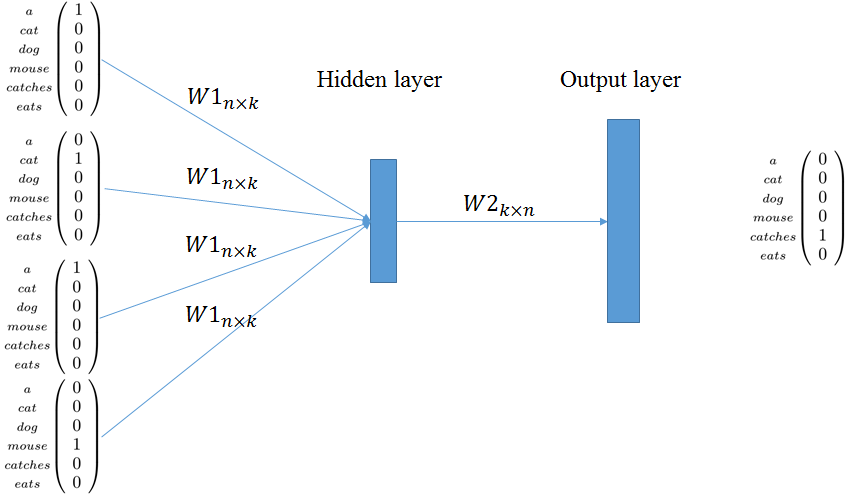
\includegraphics[width=\textwidth]{cbow-model}
	\source{ \cite{cbow_image}}
	\caption{Beispiel des \ac{cbow}-Modells.}
	\label{fig:cbow}
\end{figure}
\textit{fastText} erweitert diese Vorgehensweise und nutzt Teilwortinformationen, um ein Wort als Vektor darzustellen. Wörter werden in N-Grams dargestellt. \citep[vgl.][]{bojanowski2017enriching} Die Repräsentation für das Wort \textit{Estrich} mit n = 3 ist zum Beispiel \textit{<Es,est,str,tri,ric,ich,ch>}, wobei die Zeichen \textit{<} und \textit{>} als Begrenzungszeichen hinzugefügt werden, um die N-Gramms eines Wortes vom Wort selbst zu unterscheiden. Wäre also das Wort \textit{ich} im Vokabular, wird es als \textit{<ich>} dargestellt. Das neuronale Netz wird dann mit der Liste der N-Gramms inklusive dem kompletten Wort trainiert. Somit ermöglicht das Modell die gemeinsame Nutzung der Teilwortinformationen für alle Wörter \citep[vgl.][]{bojanowski2017enriching}. Zusätzlich nutzt \textit{fastText} eine hierarchische Softmax Verlustfunktion, um die Berechnung von unausgewogenen Verteilungen zu beschleunigen \citep[vgl.][]{fastText_release2016}.

\textit{fastText} hat für den Anwendungsfall folgende Vorteile:

\begin{itemize}
	\item \textit{fastText} kann mit Wörtern außerhalb des Vokabulars umgehen. Bei unbekannten Wörtern werden die Vektoren der einzelnen Char-Ngramms summiert. Es muss allerdings mindestens eines der Char-Ngrams in den Trainingsdaten vorhanden sein. \citep[vgl.][]{gensim_fastText,le2014distributed} Da sich bei diesem Konzept der Feinstrukturierung das Vokabular bei Ausführung vom Trainingsvokabular unterscheidet, ist das Verarbeiten von unbekannten Wörtern essenziell.
	\item \textit{fastText} liefert Vektordarstellungen mit fester Länge, welche für das Clustering mit zum Beispiel \ac{dbscan} nötig ist. \citep[vgl.][]{le2014distributed}
	\item \textit{fastText} liefert bessere Ergebnisse bei syntaktischen Aufgaben als zum Beispiel \textit{Word2Vec} und \textit{Bag of Words} \citep[vgl.][]{fastText_word2vec_comparison,le2014distributed}
	\item \textit{fastText} hat eine schnellere Trainingszeit als vergleichbar genaue Deep Learning Algorithmen \citep[vgl.][]{fastText_release2016}
\end{itemize}


Mit dem fertige trainierten \textit{fastText} Modell können dann Wörter in Vektoren umgewandelt werden. Bei der Vektorisierung von Materialien, die aus mehreren Wörtern bestehen, werden die Vektoren der einzelnen Wörter aufaddiert. Das ist dieselbe Vorgehensweise, wie \textit{fastText} bei neuen Worten, die nicht im Vokabular vorkommen, vorgeht \citep[vgl.][]{gensim_fastText}.

Wenn die Materialbezeichnungen vektorisiert wurden, können sie geclusterd werden. Aus einer großen Auswahl an Cluster-Algorithmen bietet sich \ac{dbscan} an. \glqq The \ac{dbscan} algorithm views clusters as areas of high density separated by areas of low density.\grqq{} \citep{scikitlearn_clustering} Der Algorithmus wurde \citeyear{Ester1996ADA} von \citeauthor{Ester1996ADA} vorgestellt und veröffentlicht. Ziel war es einen Algorithmus zu entwickeln, bei dem man wenig Fachwissen für die Bestimmung der Parameter braucht, Cluster mit beliebiger Form bekommen kann und eine gute Effizienz bei großen Datenbanken besitzt.

\ac{dbscan} müssen nur die zwei Parameter \textit{min\_samples} und \textit{eps} übergeben werden. Als erster Schritt werden alle Punkte, die inklusive sich selbst mindestens \textit{min\_samples} an Nachbarn innerhalb des Abstands von \textit{eps} haben, als Kernpunkte definiert. Alle anderen Punkte werden erstmals als Rauschen gekennzeichnet. Als Nächstes werden alle Kernpunkte, die inherhalb des Radius \textit{eps} beieinander liegen als ein Cluster definiert. Zum Schluss werden nochmal alle Rauschpunkte überprüft, ob sie nicht doch innerhalb des Radius eines Kernpunktes in einem Cluster liegen. \citep[vgl.][]{scikitlearn_clustering,Ester1996ADA} Die Anzahl der Cluster ist also abhängig von den Daten (und den Parametern) und muss nicht vorgegeben werden.
\ac{dbscan} hat also für den Anwendungsfall folgende Vorteile:

\begin{itemize}
	\item \ac{dbscan} liefert eine passende Anzahl von Clustern, abhängig von den Materialbezeichnungen. Dies ist wichtig, da die Anzahl der in eine Überkategorie zugewiesene Materialien und somit auch die Anzahl der potenziellen Clustern immer unterschiedlich ist. Das Ergebnis des Clustering wird auch direkt dem Benutzer der ORCA AVA präsentiert. Somit ist es auch nicht möglich, mit einem anderen Clustering-Algorithmus über die Anzahl von Clustern zu iterieren und das fachlich beste auszuwählen.
	\item Es müssen keine Trainingsdatensätze oder Modelle verwaltet werden.
	\item Der Algorithmus setzt die mitgegebene Bedeutung des Wortes bei der Wort-Einbettung mit \textit{fastText} um. 
\end{itemize}

Am Ende liefert \ac{dbscan} zu jedem übergebenem Material eine Zahl, die das Cluster repräsentiert. Rauschpunkte werden mit -1 zurückgegeben. Diese werden dann nicht weiter strukturiert und bleiben hierarchisch direkt unter ihrer zugewiesenen Überkategorie. Dieses Format kann für die Evaluationsbeispiele (\autoref{t:evaluation-example1} - \autoref{t:evaluation-example22}) direkt genutzt werden. Bei diesem Ergebnis fehlen für die endgültige Materialstrukturierung noch die Begriffe der Gliederungspunkte für die entstandenen Cluster. Hierfür wird der größte gemeinsame Nenner der Zeichenketten genutzt.

\chapter{Gegenüberstellung der möglichen Konzepte}
\label{c:comparison}
In diesem Kapitel werden die in \autoref{c:conception} vorgestellten Algorithmen verglichen.
Dies wird gesondert für die Textklassifizierung und die Feinstrukturierung durchgeführt. Es wird jeweils das Ergebnis ausgewertet und eine Auswahl eines Algorithmus durchgeführt.
\section{Vergleich der Textklassifizierung}
\label{c:comparison:classification}
Für die Textklassifizierung wird der beste Algorithmus der \textit{ML.NET}-Bibliothek gesucht. Zur Auswahl stehen das \textit{Maximum Entropy Model} mit \ac{sdca} oder \ac{lbfgs} als Optimierungsalgorithmus, die preview Textklassifizierungsschnittstelle basierend auf einem NAS-BERT Transformer und der One-Versus-All Ansatz mit einem binären Klassifizierer basierend auf logistischer Regression mit dem \ac{sdca} Optimierungsalgorithmus.

\subsection{Auswertung}
\label{c:comparison:classification:evaluation}
Bei der Textklassifizierung werden die Algorithmen nach den in \autoref{c:conception:classification:criteria} erläuterten Kriterien der Messbarkeit ausgewertet. Die Ergebnisse sind in \autoref{t:classification-result} zu sehen. Zusätzlich befinden sich in \autoref{t:confusionmatrix-sdca}, \ref{t:confusionmatrix-lbfgs}, \ref{t:confusionmatrix-onevsall} und \ref{t:confusionmatrix-text} die Konfusionsmatrix für jeden Algorithmus. Da nur 500 Datensätze zum Trainieren zur Verfügung stehen, konnten nur 20 \% und somit 94 Testdatensätze definiert werden. Da diese von \textit{ML.NET} zufällig ausgewählt werden, kann es zu Variationen der Ergebnisse kommen. Die in dieser Arbeit verwendeten Messdaten repräsentieren eine durchschnittliche Auswertung der Algorithmen. 

% Tabelle
\begin{table}[!ht]
	\centering
	\resizebox{\columnwidth}{!}{
		\begin{tabular}{|l|l|l|l|l|}
			\hline
			\textbf{Algorithmus} & \textbf{MicroAccuracy} & \textbf{MacroAccuracy} & \textbf{LogLoss} & \textbf{TrainingTime} \\ \hline
			\textbf{SdcaMaximumEntropy} & 0,882 & 0,910 & 0,477 & 0,245sec \\ \hline
			\textbf{LbfgsMaximumEntropy} & 0,670 & 0,591 & 1,131 & 0,243sec \\ \hline
			\textbf{TextClassification} & 0,479 & 0,292 & 5,994 & 20,229sec \\ \hline
			\textbf{OneVersusAll SdcaLogisticRegression} & 0,872 & 0,894 & 0,477 & 4,219sec \\ \hline
		\end{tabular}
	}
    \caption{Auswertung der Textklassifizierungsalgorithmen}
   	\label{t:classification-result}
\end{table}

Die Klassifizierungsalgorithmen liefern verschiedene Ergebnisse. Bei der Betrachtung der Genauigkeit schneidet \textit{SdcaMaximumEntropy} mit einer Genauigkeit von 88,2 \% am besten ab, dicht verfolgt von \textit{OneVersusAll} mit 87,2 \%. \textit{LbfsgMaximumEntropy} und die \textit{TextClassification} haben dagegen nur eine Genauigkeit von 67 \% bzw. 48 \%. In den Konfusionsmatrizen dieser beiden erkennt man, dass vor allem die Klassen \textit{Mineralisch} und \textit{Metall} mit einer schlechten Genauigkeit von 43 \% bzw. 35 \% abschneiden. Mineralische Materialien wurden hier zwar meistens (96 \%/87 \%) richtig zugeordnet.  Materialien vieler anderer Klassen wurden aber auch in diese beiden Klassen bei der Vorhersage zugewiesen. Bei \textit{SdcaMaximumEntropy} und \textit{OneVersusAll} ist das ähnlich zu beobachten. Mineralische Materialien werden bei beiden Modellen zu 92 \% richtig klassifiziert. Hier ist die Genauigkeit aller mineralisch zugeordneten Materialien bei 76\%. Der LogLoss ist bei diesen beiden Modellen auch mit 0,477 deutlich niedriger als bei den anderen Algorithmen.

Die Maximum Entropy Modelle scheiden bei der Trainingsdauer am besten ab. Mit ca. 0,24 Sekunden ist die Trainingszeit bei beiden Modellen zu vernachlässigen und kann theoretisch sogar nach jedem neu klassifizierten Datensatz direkt durchgeführt werden. Da der \textit{OneVersusAll} Algorithmus mehrere binäre Modelle trainieren muss, braucht er mit 4,2 Sekunden deutlich länger. Das \textit{TextClassification} Modell braucht ganze 20 Sekunden, um die 406 Datensätze zu trainieren.

\subsection{Auswahl eines Algorithmus}
\label{c:comparison:classification:selection}
Die Wahl des Textklassifizierungsalgorithmus fällt eindeutig auf \textit{SdcaMaximumEntropy}. Mit einer Genauigkeit von 88,2 \% wurde ein nutzbares Ergebnis erzielt. Zusätzlich ist es der Algorithmus mit der kürzesten Trainingsdauer. Auch wenn der \textit{OneVersusAll} Ansatz auf eine ähnliche Genauigkeit kommt, dauert das Training deutlich länger und das gespeicherte Modell braucht mehr Speicher, als das gespeicherte \textit{SdcaMaximumEntropy} Modell. 
Zusätzlich wurde das \textit{SdcaMaximumEntropy} Modell dem Projektmanagement vorgestellt und fachlich evaluiert. Das Ergebnis wurde als fachlich brauchbar eingestuft und kann somit für die Textklassifizierung genutzt und integriert werden.

Um die Anzahl der Trainingsdaten besser einschätzen zu können, wird in \autoref{fig:accuracy-graph} der Genauigkeitsverlauf für die jeweilige Anzahl der Trainingsdaten gezeigt. Man sieht eine abflachende Kurve, die andeutet, dass der Anstieg der Genauigkeit bei noch größerer Trainingsdatenanzahl immer kleiner wird. Mit mehr Trainingsdaten wird allerdings auch die Anzahl der Testdaten größer und somit auch die Genauigkeit konstanter. Es wäre somit langfristig noch sinnvoll, die Trainingsdaten zu erweitern.

\begin{figure}[h]
	\centering
	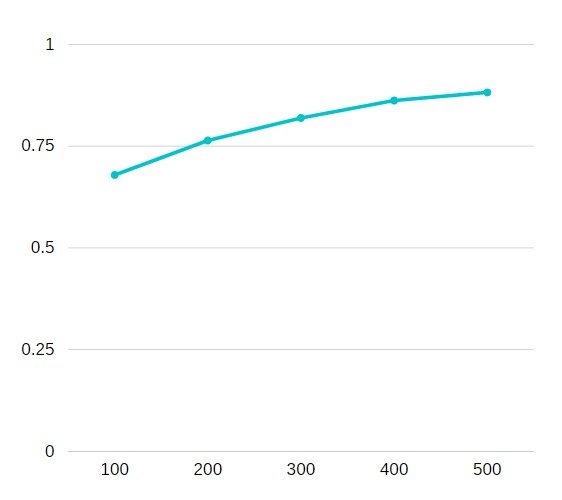
\includegraphics[width=0.7\textwidth]{accuracy-graph}
	\caption[Genauigkeit des SdcaMaximumEntropy-Modells]{Genauigkeit des SdcaMaximumEntropy-Modells für die jeweilige Trainingsdaten-Anzahl. (Durchschnittswerte von 100 Trainingsdurchläufen bei einem Testsplit von 0.2)}
	\label{fig:accuracy-graph}
\end{figure}

\section{Vergleich der Feinstrukturierung}
\label{c:comparison:fine-structuring}
Bei der Feinstrukturierung wird zwischen dem fertig trainierten GPT-Modell von OpenAi und einem selbst implementieren Vorgehensweise mit \textit{fastText} und \ac{dbscan}-Clustering verglichen.
\subsection{Auswertung}
\label{c:comparison:fine-structuring:evaluation}
Die Algorithmen für die Feinstrukturierung werden zuerst nach den Kriterien der Messbarkeit aus \autoref{c:conception:fine-structuring:criteria} ausgewertet.
Das Ergebnis ist in \autoref{t:evaluation-example1} bis \autoref{t:evaluation-example22} mit eingetragen. -1 bedeutet, dass das Ergebnis nicht nutzbar ist, da zum Beispiel die Materialbezeichnung vom Algorithmus verändert wurde. Zusätzlich ist in \autoref{t:structuring-result} eine akkumulierte Auswertung zu sehen, bei der die Ergebnisse in folgende Klassen zusammengefasst wurden. \textit{Richtig} heißt, dass das Ergebnis mit dem erwarteten Ergebnis übereinstimmt. \textit{Teilweise Richtig} bedeutet, dass manche Materialien zwar nicht zugewiesen wurde, aber es keine fachlich falsche Zuweisung enthält. Dieses ist laut dem Produktmanagement als ausreichendes Ergebnis für die Feinstrukturierung zu sehen.  Bei \textit{Falsch} wurde ein oder mehrere Materialien falsch zugewiesen, oder das Ergebnis war nicht für die Weiterverarbeitung nutzbar. 

\begin{table}[!ht]
	\centering
	\begin{tabular}{|l|l|l|}
		\hline
		\textbf{} & \textbf{fastText \& DBSCAN} & \textbf{OpenAI} \\ \hline
		\textbf{Richtig} & 9 & 5 \\ \hline
		\textbf{Teilweise Richtig} & 6 & 10 \\ \hline
		\textbf{Falsch} & 7 & 7 \\ \hline
	\end{tabular}
	\caption{Auswertung der Feinstrukturierung in \textit{Richtig}, \textit{Teilweise Richtig}, und \textit{Falsch}}
	\label{t:structuring-result}
\end{table}

\noindent Vorteile von \textit{fastText} \& \textit{\ac{dbscan}}:
\begin{itemize}
	\setlength\itemsep{0em}
	\item Besseres Ergebnis bei der Auswertung der Evalutaionsbesipiele (siehe \autoref{t:structuring-result})
	\item deterministischer Algorithmus liefert für gleiche Eingabe immer das gleiche Ergebnis
	\item keine zusätzlichen Kosten
	\item Gute Interpretierbarkeit des Algorithmus
\end{itemize}
Nachteile von \textit{fastText} \& \textit{\ac{dbscan}}:
\begin{itemize}
	\setlength\itemsep{0em}
	\item Erhöhter Aufwand durch das Pflegen und Verbessern des selbst trainierten \textit{fastText}-Modells
	\item Clustert teilweise nach irrelevanten Worten. (z.B.: matt, verputzt)
\end{itemize}
Vorteile von \textit{ChatGPT}:
\begin{itemize}
	\setlength\itemsep{0em}
	\item Kein Wartungsaufwand von selbst trainierten Modellen.
	\item Liefert fachlich meistens ein fachlich richtiges Ergebnisse.
\end{itemize}
Nachteile von \textit{ChatGPT}:
\begin{itemize}
	\setlength\itemsep{0em}
	\item Verändert Materialbezeichnungen, was das Ergebnis für als Kostengliederung nicht brauchbar macht. Aus \textit{Stahl matt} wird zum Beispiel \textit{1.1 Stahl} und \textit{1.1.1 matt}
	\item Die Ausgabe ist trotz \textit{Temperature} von 0 nicht deterministisch. Das senkt in Kombination mit der Veränderung von Begriffen die Interpretierbarkeit des Algorithmus.
	\item Die Form der Ausgabe als Zeichenkette und mögliche Variationen in der Struktur der Ausgabe kann zu Fehlern beim Abbilden in die Objektstruktur führen.
	\item Zusätzlicher Kostenaufwand von 0.002 \$ pro 1000 Tokens
\end{itemize}
\subsection{Auswahl eines Algorithmus}
\label{c:comparison:fine-structuring:selection}
Für die Feinstrukturierung kommt nur \textit{fastText} \& \textit{\ac{dbscan}} als einzige Option infrage. Das fachliche Ergebnis der jeweiligen Strukturierung lässt beide Optionen für die Feinstrukturierung zu. \textit{fastText} \& \textit{\ac{dbscan}} scheiden bei den Evaluationsbeispielen aber auch schon besser ab. Die beiden Algorithmen unterscheiden sich vor allem in der Interpretierbarkeit (\autoref{def:interpretability}). Die genannten Nachteile von \textit{ChatGPT} führen schnell zu fehlender Interpretierbarkeit und somit zu Misstrauen gegenüber der Programmerweiterung.
Vor allem die Kombination der einzelnen Nachteile lässt manche Ergebnisse willkürlich erscheinen. Zusätzlich können mit \textit{ChatGPT} oft kein Ergebnis zur Verfügung gestellt werden, da nach der Veränderung von Materialbezeichnungen die ursprünglichen Materialien nicht mehr nachvollzogen werden können.
\textit{fastText} \& \textit{\ac{dbscan}} schneiden in der Interpretierbarkeit gut ab. Das entsteht durch deterministische Ergebnisse und nachvollziehbares Clustering. Das Zusammenfassen von mehreren Materialien in ein Cluster kann immer, auch bei einem fachlich falschen Ergebnis, nachvollzogen und eine Logik hinter der Strukturierung gefunden werden. Durch die bessere Interpretierbarkeit wird \textit{fastText} \& \textit{\ac{dbscan}} als Algorithmus für die Feinstrukturierung festgelegt.

\chapter{Praktische Umsetzung}
\label{c:implementation}
In diesem Kapitel wird die Umsetzung der ausgewählten Algorithmen und Bibliotheken beschrieben. Zuerst wird die Implementierung des Services und der Python-Interop gezeigt. Danach geht es um die konkrete Implementierung der Materialstrukturierung.

\section{Implementierung des ASP.NET Services}
\label{c:implementation:service}
Die Realisierung als ASP.NET Service ist eine Anforderung der \glqq ORCA Software GmbH\grqq{}. Für das Erstellen eines neuen Services gibt es ein fertiges Projekttemplate, welches nur umbenannt werden muss. Die Vorlage liefert eine einheitliche Projektstruktur und zeigt den Aufbau des Services anhand der Implementierung eines Beispiels. Die neu genannte \textit{ MaterialStructurizationApi} hat zwei verschiedene \ac{rest}-Controller.
Diese teilen sich, wie im Anwendungsfalldiagramm (\autoref{fig:usecasediagramm}) zu sehen, in die Schnittstellen für die ORCA AVA Benutzer und die ORCA internen Schnittstellen auf. In den Controllern werden die \ac{rest}-Schnittstellen-Methoden definiert. Dazu zählt die Art der Anfragemethoden, die Request-\ac{url} oder auch die möglichen Antwort-StatusCodes. Service interne Logik wird im \code{MaterialService} organisiert. Hier werden die \acp{dto} in Entitäten umgewandelt und die Aufrufe auf die entsprechenden weiteren themenspezifischen \code{Services} oder Datenzugriff-Repositories weitergeleitet. Am Ende werden Rückgabewerte wieder in entsprechende \acp{dto} abgebildet und an den Controller zurückgegeben. Ein Beispiel ist in \autoref{lst:materialservice} zu sehen. Die Methode ist für die Materialstrukturierung zuständig. Sie bekommt die Liste von Manualbezeichnungen und eine \code{bool}, welcher bestimmt, ob die Feingliederung durchgeführt werden soll, übergeben. Nach der Parameterprüfung werden Duplikate aus der Materialliste entfernt und danach in Zeile 8 über das \code{MaterialRepository} neue Materialien dem Trainingsdatensatz für die Klassifizierung hinzugefügt. Danach wird der \code{MaterialStructurizerService} aufgerufen, der sich dann um die Logik der Strukturierung kümmert.

Repositories kapseln den Datenzugriff über Interfaces. So ist die Logikimplementierung in den Services unabhängig von der Implementierung des Datenbankzugriffs. Der Datenbankzugriff wird in den Repositories mit der Object-Relation-Mapper Bibliothek \textit{EntityFramework} implementiert. Es wird der Model-First Ansatz verwendet, bei dem zuerst die Objektstruktur im C\#-Code definiert wird und daraus automatisiert die Datenbank generiert wird.

\section{Python-Interop}
\label{c:implementation:python-interop}
Für die Implementierung einiger Komponenten wird Python als Programmiersprache benötigt. Der Webservice wird allerdings mit ASP.NET implementiert. Um die Kommunikation zwischen .NET und Python zu vereinfachen, wird das Nuget-Packet \code{pythonnet} verwendet. Die Bibliothek vereinfacht es, Python-Code aus dem C\#-Code auszuführen und verschiedene Python-Variablen auszulesen oder diesen Werte zuzuweisen. Um den Python-Interop nutzen zu können, muss eine lauffähige Python-Umgebung in der Ausführungsumgebung installiert sein. Der Python-Interop ist in mit dem Interface \code{IKiExecuter} gekapselt und lässt so eine eventuelle C\# Ablösung der Python-Komponenten in der Zukunft einfach integrieren. In \autoref{lst:pythonnet} ist der Python-Code Aufruf für das Preprocessing zu sehen. Nachdem die Python-Engine initialisiert wird, kann der Python-Variable ein Wert zugewiesen werden. Dann wird das Skript \textit{preprocess.py} (\autoref{lst:preprocess}) über den Namen aufgerufen und danach die Python-Variable \code{material\_preprocessed}, in welcher am Ende des Python-Skripts das Ergebnis steht, wieder ausgelesen.

\lstinputlisting[language={[Sharp]C}, caption={Python-Interopt Aufruf für das Preprocessing}, style={csharp}, label={lst:pythonnet}]{Pythonnet.cs}

Zusätzlich löst \textit{pythonnet} das Problem, dass das Pythonskript zur Feinstrukturierung nicht immer wieder das \textit{fastText}-Modell neu in den Speicher laden muss. Durch die Möglichkeit Python-Variablen zuzuweisen und auszulesen, ist es auch möglich das \textit{fastText}-Modell initial beim Starten des Services in den Speicher zu laden. Das macht das Ausführen der Feinstrukturierung sehr viel performanter und erst produktiv einsetzbar.

Für die Entwicklung der Pythonskripte wird die Logik immer in eine Methode ausgelagert. Mit der Zeile \code{if \_\_name\_\_ == "\_\_main\_\_":} wird der darauf folgende Code beim initialen Aufrufen des Skriptes ausgeführt. Mit einem Try-Except-Block wird überprüft, ob durch \textit{pythonnet} die Eingabevariable schon initialisiert wurde. Ansonsten kann beim Debuggen ein Wert über die Kommandozeile eingetragen werden. Somit kann für alle Konstellationen immer nur ein Skript verwendet werden. Das ganze Skript inklusive der definierten Methoden können dann mit \textit{pythonnet} im C\#-Code und aber auch autark im Debug-Modus ausgeführt werden. (Beispiel:  \autoref{lst:preprocess})

\section{Implementierung der Materialstrukturierung}
\label{c:implementation:structuring}
Die Implementierung der Materialstrukturierung teilt sich ähnlich wie in \autoref{c:conception} auf. Zuerst geht es um das Erstellen einer Datengrundlage, dann um die Implementierung des Preprocessings. Anschließend wird das Textklassifizierungsmodell vorgestellt. Für die Feinstrukturierung wird am Ende noch die Implementierung für \textit{fastText} und \ac{dbscan} erläutert.
\subsection{Erstellen einer Datengrundlage}
\label{c:implementation:data} 
Die Datengrundlage entstand durch das Extrahieren der Materialangaben (wie in \autoref{c:conception:architecture:ifc-material-extraction} beschrieben) aus verschiedenen \ac{ifc}-Dateien. Hierzu standen über 500 verschiedene Dateien zur Verfügung. Die daraus entstandenen Materialbezeichnungen wurden über eine \ac{http}-PUT Anfrage in einem \ac{sql}-Server mit dem in \autoref{fig:db-scheme} abgebildetem Schema persistiert. Die Liste dieser Materialien wurden anschließend manuell gefiltert. In vielen \ac{ifc}-Dateien werden die Möglichkeiten der Materialangabe noch nicht gut genutzt. Deshalb waren viele Materialangaben nicht aussagekräftig, um sie als Trainingsdaten für die Textklassifizierung zu nutzten. Am Ende standen circa 500 unterschiedliche Materialbezeichnungen zur Verfügung.
Um die Daten anschließend zu klassifizieren, wurde ein Klassifizierungs-Service mit Oberfläche implementiert (siehe  \autoref{fig:classification-service}). Dieser stand im internen Firmennetzwerk zur Verfügung, sodass ausgewählte Mitarbeiter die Materialien klassifizieren konnten. Die dafür benötigten Methoden standen über den \code{InhouseMaterialController} der \textit{MaterialStructurizationApi}, welcher die internen ORCA-Schnittstellen bietet, zur Verfügung. Somit wurden über 480 klassifizierte Datensätze geschaffen. Die Verteilung der Klassifizierung ist in \autoref{fig:distribution-diagramm} zu sehen.

\subsection{Implementierung des Preprocessings}
\label{c:implementation:preprocess}
Das Preprocessing für die Textklassifizierung wurde in Python implementiert.
Das Vorgehen wurde schon in \autoref{c:conception:architecture:preprocessing} erläutert. Die Implementierung des Pythonskripts ist in \autoref{lst:preprocess} zu sehen. Das Preprocessing basiert größtenteils auf der Textverarbeitung mit Regex. Mit dem Regex \code{[A-Za-z0-9üäöÜÄÖßóåéèÉÈÓ/]} werden alle Sonderzeichen bis auf  \glqq /\grqq{} aus dem String entfernt. Bei der Maßangabe mussten aufgrund der unterschiedlichen Verarbeitung bei gleicher Eingabe des Python-Package \code{re} bei \code{re.findall(...)} \code{re.sub(...)} mehrere Regex definiert werden. Zuerst werden dreidimensionale Maße im Materialstring gesucht. Wenn keine vorhanden sind, werden zweidimensionale Maße entfernt. Ansonsten wird mit einem zusätzlichen Regex die dreidimensionalen Maßangaben entfernt. Am Ende wird eine Liste von Strings aus dem Materialstring gefiltert und überschüssige Leerzeichen mit \code{strip()} entfernt. 

Wie in \autoref{fig:db-scheme} zu sehen ist, werden die vorverarbeiteten Materialien in der Datenbank persistiert. Immer wenn ein neues Material in die Datenbank geschrieben wird, wird das Preprocessing gestartet. Das bietet die Möglichkeit direkt nach dem Klassifizieren eines Materials, das Textklassifizierungsmodell ohne vorheriges Preprocessing aller Datensätze neu trainieren zu können. Dadurch verringert sich die Ausführungszeit des Trainingsprozesses und es kann direkt auf das aktualisierte Modell zugegriffen werden.

\subsection{Training des Textklassifizierungsmodells}
\label{c:implementation:classification-training}
\textit{ML.NET} bietet einem für jedes Machine-Learning-Model eine ähnliche Codestruktur. Diese ist in \autoref{fig:mlnet-workflow} aufgezeigt. Parallel dazu ist in \autoref{lst:ml-net} ein leicht vereinfachter Codeausschnitt für das Trainieren des Materialklassifizierungsmodells zu sehen. Im Trainingsprozess wird nach dem Laden der Trainingsdaten in den Trainingskontext die Pipeline definiert. Mit der \code{Append()}-Methode können verschiedene Schritte der Pipeline hinzugefügt werden. Im ersten Schritt werden die Texte normalisiert und mit Bag-of-words und N-Grams in Vektoren umgewandelt. Als Nächstes wird der \code{SdcaMaximumEntropy} als Klassifizierungsalgorithmus hinzugefügt. Mit \code{MapKeyToValue()} werden die Schlüsseltypen in ihre ursprünglichen Werte zurück umgewandelt.
Mit der \code{Fit()}-Methode wird die Trainingspipeline ausgeführt und ein Modell erzeugt. Mit \code{Evaluate} kann das Modell dann analysiert und bewertet werden. Die Methode liefert einige Kennzahlen, wie die Genauigkeit sowie den \code{LogLoss}, welche in \autoref{c:comparison:classification:evaluation} schon für die Auswertung verwendet wurden. Um ein Modell zu persistieren, kann es mit \code{Save()} als ZIP-Datei gespeichert werden. Um das Modell wieder nutzen zu können, wird das Modell mit \code{Load()} geladen und eine \code{PredictionEngine} erzeugt. Mit diesem Objekt kann die \code{Predict()}-Methode ausgeführt werden, welche die Vorhersage für die Materialüberkategorie liefert.

\lstinputlisting[language={[Sharp]C}, caption={vereinfachter Code für das Trainieren des Materialklassifizierungsmodells mit \textit{ML.NET} }, style={csharp}, label={lst:ml-net}]{MaterialClassification.cs}

\subsection{Training des \textit{fastText} Modells}
\label{c:implementation:embedding-training}
Für das Trainieren des \textit{fastText}-Modells wird die Python-Bibliothek \textit{Gensim}  \citep[vgl.][]{rehurek_lrec} verwendet. Die Bibliothek implementiert verschiedene Vektorisierungsalgorithmen, wie zum Beispiel \textit{Word2Vec}, \textit{EnsembleLDA} aber auch \textit{fastText}.

Über eine interne Schnittstelle wurden alle \ac{ade}-Texte in Textdateien gespeichert. Der Trainingsablauf wurde in drei Skripte aufgeteilt. Das Skript \textit{fasttext\_prepare.py} liest die Katalogtexte ein und führt das in \autoref{c:conception:fine-structuring:dbscan} erläuterte Preprocessing aus.
Das Skript \textit{fasttext\_train.py} liest die vorverarbeiteten Texte wieder ein, teilt sie in Sätze ein und generiert Tokens aus jedem Satz. Bei der Aufteilung in Sätze werden Abkürzungen, in denen ein Punkt vorkommt, beachtet und führen zu keinem eigenen Satz. Anschließend wird ein \textit{fastText}-Modell initialisiert, trainiert und am Ende gespeichert.

Mit dem dritten Skript \textit{fasttext\_test.py} kann man das trainierte Modell fachlich bewerten. Mit der Methode \code{most\_similar(positive=[word],topn=100)} werden die 100 ähnlichsten Wörter zu einem Wort ausgegeben. Da der Algorithmus \ac{dbscan} mit der Dichte von Punkten und somit der \glqq Ähnlichkeit\grqq{} von Worten funktioniert, ist diese Methode eine gute Möglichkeit das Modell fachlich zu evaluieren und testen.

\subsection{Ausführen der Feinstrukturierung}
\label{c:implementation:clustering}
Die Feinstrukturierung wird im Pythonskript \textit{dbscan\_structurize.py} ausgeführt und kann parallel abgearbeitet werden. Nachdem das \textit{fastText}-Modell geladen wurde, werden für jede Überkategorie mit mehr als zwei Materialien ein Threat für die Feinstrukturierung gestartet. Den folgenden Ablauf kann man in zwei Schritte einteilen. Da die Begriffe schon bei der Textklassifizierung durch das Preprocessing gelaufen sind, ist das nicht mehr nötig. Der erste Schritt ist das Vektorisieren der Materialbezeichnungen. Hier werden die Begriffe mit \code{tokenize()} in die einzelnen Wörter geteilt und dann der Vektor durch die Summe aller Wortvektoren ermittelt. Hierzu werden die Wörter nacheinander mit dem \textit{fastText}-Modell in Vektoren umgewandelt und dann aufaddiert. Danach beginnt der zweite Schritt des Clusterings. Hierzu wird die \ac{dbscan}-Implementierung von \textit{scikit-learn} \citep{scikit-learn} genutzt. Der \ac{dbscan}-Parameter \textit{min\_samples} wird auf 2 gesetzt, damit Cluster ab zwei Materialien entstehen können. Über den Parameter \textit{eps} wird von 0,5 bis 5 in 0,1-Schritten iteriert. Da jede Ausführung von \ac{dbscan} andere Eingabevektoren hat, muss auch der Parameter \textit{eps} immer anders gewählt werden, um das optimale Ergebnis zu bekommen. Das optimale Ergebnis bedeutet, möglichst viele verschiedene Cluster zu erhalten und dabei den Median der Anzahl der Rauschpunkte bei dieser Anzahl von möglichst vielen Clustern zu haben. Bei der Iteration über den Parameter kann das optimale Ergebnis, durch Evaluieren der jeweiligen Clusteranzahl und Anzahl von Rauschpunkten, ermittelt werden. Der Startwert und Endwert haben sich durch Testen als passende Werte ergeben, sodass das optimale Ergebnis immer innerhalb des Bereiches liegt. Am Ende wird das optimale Ergebnis an den ASP.NET Service zurückgegeben. Dort wird der Rückgabewert in eine passende Objektstruktur abgebildet und als \ac{dto} als \ac{http}-Response zurückgegeben.

\chapter{Maßnahmen zur Qualitätssicherung}
\label{c:qs}
Dieses Kapitel beinhaltet Clean Code Prinzipien und technische Hilfsmittel sowie Unit-Tests, um die Qualitätssicherung sicherzustellen.

\section{Clean Code}
\label{c:qs:cleancode}
\begin{definition}[Clean Code]
	\label{def:clean-code}
	\glqq Clean code is simple and direct. Clean code reads like well-written prose. Clean code never obscures the designer’s intent but rather is full of crisp abstractions and straightforward lines of control. - Grady Booch author of Object Oriented Analysis and Design with	Applications\grqq{} \citep[p.~8]{martin2009clean}
\end{definition}
Um die Qualitätssicherung bereits vor der Ausführung von Tests sicherzustellen, gilt es gewisse Clean Code Konventionen adäquat anzuwenden.
Durch die Verwendung von SonarCloud und SonarLint wird die Anwendung der Code Konventionen sichergestellt. SonarLint führt Analysen während des Programmierens durch und gibt dementsprechend Warnungen bzw. Fehler aus. Welche Konventionen SonarLint analysiert, ist über eine Konfigurationsdatei steuerbar. So ist der Entwickler gezwungen, schon beim Entwickeln die verschiedenen Aspekte von Clean Code zu beachten. Zusätzlich läuft mit SonarCloud eine statische Codeanalyse in der Build-Pipeline. Diese verhindert, dass unkonventioneller Code eingecheckt werden kann. Für den entwickelten Service wurden am Ende der Entwicklung keine Code Smells gefunden. Auch ein Security-Scanner ist in die Build-Pipeline integriert, um Sicherheitsrisiken zu erkennen. Außerdem werden Code Reviews bei einem Pull Request durchgeführt. Durch das Vier-Augen-Prinzip werden so zusätzlich Fehler und Code Smells reduziert.

\section{Technische Hilfsmittel}
\label{c:qs:technical_aids}
Bei der Durchsetzung von Maßnahmen der Qualitätssicherung wurden technische Hilfsmittel verwendet. Diese sind Visual Studio, Visual Studio Code, Azure Data Studio und Azure DevOps. Auf diese wird in diesem Abschnitt eingegangen. Alle benötigten Lizenzen werden von der \glqq ORCA Software GmbH\grqq{} zur Verfügung gestellt. Die Implementierung des ASP.NET-Service wird mit Visual Studio Enterprise 2022 von Microsoft durchgeführt. Die Pythonskripte wurden mit Visual Studio Code implementiert. Mit der \glqq Python\grqq{} Erweiterung kann der entwickelte Code direkt ausgeführt und gedebugged werden.
Für das Verwalten der \ac{sql}-Datenbanken wird Azure Data Studio genutzt. Beim Entwickeln wird eine lokale Datenbank verwendet. Diese wird mit \textit{EntityFramework} und dem Code-First Ansatz automatisch erzeugt. Mit \ac{sql}-Statements über Azure Data Studio können die Daten aber manuell eingesehen oder editiert werden.

Das Projektmanagement (siehe \autoref{c:basics:project-management}) wird mit Azure DevOps umgesetzt. In diesem werden theoretische Arbeiten durchgeführt, als auch alle praktischen Aufgaben, damit alle Daten an einem zentralen Ort sind. Die Plattform hilft dabei, Maßnahmen zur Qualitätssicherung zu treffen und umzusetzen. Zu Beginn wurde alle bekannten Aufgaben in Pakete unterteilt. Diese Aufgaben wurden schriftlich formuliert und anschließend als User Stories und Tasks in Azure DevOps eingetragen. Im Sprint Planning wurden dann dementsprechende User Stories dem Sprint zugewiesen. Nachdem ein neuer Quellcode verfasst oder alter Quellcode geändert wurde, wurde dieser auf den Azure DevOps Server geladen und mit dem zugehörigen Arbeitselement verknüpft. Bevor der Stand in das Remote Repository integriert wird, startet eine Pipeline. Diese kompiliert den neuen oder geänderten Quellcode, führt die genannten Analysen aus und testet, ob alle Tests erfolgreich durchlaufen. Die Nutzung ist lizenzpflichtig.

\section{Tests und Abnahme}
\label{c:qs:tests}
Um einen funktionsfähigen Service zur Verfügung stellen und sicher weiterentwickeln zu können, muss dieser ausreichend getestet werden. Für den ASP.NET-Service werden dafür Unit-Tests implementiert. Diese werden auch in der Build-Pipeline geprüft. Getestet wird vor allem die Controllerlogik, Pythonlogik und Repositorylogik. Controller können mithilfe von Mocking der genutzten Repositories und Services realisiert werden. Die Pythonskripte wurden inklusive des Python-Interop mit der Klasse \code{IPythonKiExcuter} getestet. Somit muss keine weitere Unit-Test-Bibliothek verwendet werden. Beim Testen von Repositories wird mithilfe des \textit{In-memory Provider} von \textit{EntityFramework} die Datenbank im Arbeitsspeicher emuliert. So können Zugriffe während des Tests durchgeführt werden, ohne eine echte Datenbank zu benutzten.

Da im Rahmen dieser Arbeit die Nutzung der Materialstrukturierung temporär nur in einem Draft-Projekt implementiert ist und noch keine komplette Integration in die ORCA AVA stattgefunden hat, gibt es eine fachliche Abnahme der Strukturierung der Materialien. In einem Meeting mit dem Entwicklungsleiter und dem Projektmanagement wurde das Ergebnis der Strukturierung durchgesprochen und die zukünftige Verwendung diskutiert. Die Implementierung als Kostengliederungsimport ist weiterhin vorgesehen und wird in \autoref{c:closing:integration} behandelt.

\chapter{Abschluss}
\label{c:closing}
In diesem letzten Kapitel wird ein Fazit gezogen, die Integration in die ORCA AVA aufgezeigt und ein Ausblick gegeben.

\section{Fazit}
\label{c:closing:conclusion}
In diesem Abschnitt werden die Ergebnisse der Forschung und praktischen Arbeit zusammengefasst, interpretiert und überprüft, ob das Ziel der Arbeit erreicht wurde. Am Ende werden Beschränkungen der Arbeit aufgezeigt.

\subsubsection{Zusammenfassung der Ergebnisse}
Zu Beginn wurde die Arbeit motiviert und die Problemstellungen definiert. Dafür wurde das Konzept erarbeitet, einen Webservice bereitzustellen, der die Materialstrukturierung in den drei Schritten ausführt. Diese sind das Preprocessing, die Textklassifizierung und die Feinstrukturierung eingeteilt. Für die Materialstrukturierung wurden dazu zu den Anforderungen passende Algorithmen verglichen und ausgewählt. Diese wurden nach den jeweiligen Kriterien der Messbarkeit und in der fachlichen Abstimmung mit dem Produktmanagement evaluiert. Für die Textklassifizierung und die Feinstrukturierung wurde jeweils ein passender Algorithmus gefunden. Die funktionalen Anforderungen wurden mit einem \ac{rest}full ASP.NET Service realisiert. Dieser führt mithilfe von Python-Interop die Materialstrukturierung durch. Die Textklassifizierung wird mit \textit{ML.NET} und einem Maximum Entropy Modell mit dem \ac{sdca}-Optimierungsalgorithmus durchgeführt. Bei der Feinstrukturierung stellte sich das Nutzen von \ac{dbscan} mit einer voraus liegenden \textit{fastText}-Vektorisierung als passend heraus. Die Daten für die Strukturierung werden in einer SQL-Datenbank persistiert. Zusätzlich entstand ein Draftprojekt, um den Service visuell ansteuern zu können. Dafür wurde die Extraktion aller Materialien aus einer \ac{ifc}-Datei für den IFC Manager implementiert. Die Maßnahmen der Qualitätssicherung wurden erläutert.

\subsubsection{Zielerreichung}
Zu Beginn der Arbeit wurde unter \autoref{c:intro:target} ein Ziel mit der SMART Methode definiert. Die für das Ziel definierten Anforderungen konnten durch die theoretische Konzeption in \autoref{c:conception}, die Gegenüberstellung der Algorithmen in \autoref{c:comparison} und die Implementierung in \autoref{c:implementation} umgesetzt werden. Auch die Maßnahmen zur Qualitätssicherung wurden umgesetzt und verifiziert. Bei der Evaluation wurden die Kriterien der Messbarkeit beachtet. Die Evaluation, Auswahl und Implementierung lieferten ein brauchbares Ergebnis für die Strukturierung der Materialien, welches vom Produktmanagement freigegeben wurde. Ein Draftprojekt wurde vollständig erstellt. Somit wurde das definierte Ziel der Arbeit vor Ablauf der Zeitbegrenzung erreicht.

\subsubsection{Textklassifizierung}
Die Textklassifizierung mit \textit{ML.NET} und einem Maximum Entropy Modell mit dem \ac{sdca}-Optimierungsalgorithmus lieferte trotz \autoref{p:shorttext} (Materialien sind nur Stichpunkte aus wenigen Worten) mit einer Genauigkeit von 88 \% ein gutes Ergebnis. Mit der Erweiterung der Trainingsdaten kann das Modell noch robuster und auch genauer trainiert werden. Die Implementierung in Python war hier nicht nötig und die Bibliothek \textit{ML.NET} bietet ausreichende Möglichkeiten an, die Textklassifizierung durchzuführen.

\subsubsection{Feinstrukturierung}
Für die Feinstrukturierung beweist sich das Nutzten einer domänenspezifischen Lösung. Das Trainieren eines \textit{fastText}-Modells mit Ausschreibungstexten aus der Baubranche bietet dem simplen Clustering-Algorithmus \ac{dbscan} es, nach der Bedeutung eines Wortes zu strukturieren. Somit wurde \autoref{p:shorttext} und \autoref{p:technical-term} gelöst und ein fachlich nutzbares Ergebnis erzielt. Auch wenn das manuelle Testen des \textit{fastText}-Modells mit der \code{most\_similar()}-Methode kein gutes Ergebnis versprach, war das Ergebnis beim Clustering fachlich nutzbar. Die Ähnlichkeit der Worte im \textit{fastText}-Modell sind für das Ergebnis nicht wichtig.

\subsubsection{Beschränkungen der Arbeit}
Neben den behandelten Algorithmen und Bibliotheken wurden weitere Möglichkeiten nur sporadisch untersucht und getestet. Eine erste Recherche hat auf die in der Arbeit untersuchten Lösungen hingewiesen. Alle Möglichkeiten zu analysieren würde über den Rahmen der Arbeit hinausgehen. Falls das Ergebnis der Gegenüberstellung aus Gründen in der Zukunft nicht mehr infrage kommt, können weitere Möglichkeiten wieder aufgegriffen und in Betracht gezogen werden. Zusätzlich lag der Fokus auf dem Finden passender Algorithmen. Es wurde in der Codebasis der ORCA AVA nur die Möglichkeit bereitgestellt, alle Materialien aus einer \ac{ifc}-Datei zu extrahieren. Die Programmerweiterung der Materialkostengliederung wurde nicht komplett implementiert. In \autoref{c:closing:integration} wird diese Integration beschrieben und ein Vorschlag geliefert.

\section{Integration in die ORCA AVA}
\label{c:closing:integration}
Da der Service vollumfänglich implementiert ist und das Ergebnis der Strukturierung gut genug ist, kann als nächstes die Integration in die ORCA AVA beginnen. Technisch ist eine Kostengliederung als Modell im C\# Code definiert. Der Aufbau bildet die Baumstruktur über eine Referenz zur ParentNode und mehreren ChildrenNodes ab. Das Model kann über die ORCA AVA interne Middleware in der Datenbank persistiert werden. Die persistierten Kostengliederungen werden dann in entsprechenden Programmteilen angezeigt. So müssen nach der generierten Kostengliederungs-Struktur die strukturierten Materialbezeichnungen in die C\# Objektstruktur abgebildet werden. So wird nach dem Import die erstellte Kostengliederung automatisch in der Oberfläche angezeigt und kann für Kostenauswertungen genutzt werden. Neben dem Import einer Materialkostengliederung wird nebenbei ein Import einer Raumkostengliederung aus einer \ac{ifc}-Datei implementiert, welcher diese Vorgehensweise bereits implementiert. Die Implementierung muss somit nur bei der Beschaffung der Daten aus der \ac{ifc}-Datei, auf den schon implementieren \code{MaterialManager} zugreifen. In der Oberfläche soll der Import dann über das Kontextmenü \textit{Neu} im Programmteil der Kostengliederung zur Verfügung gestellt werden. 

\section{Ausblick}
\label{c:closing:outlook}
In diesem Abschnitt wird ein Ausblick auf die Programmerweiterung der Materialstrukturierung gegeben. Für die Optimierung der Materialstrukturierung, können bei der Textklassifikation mit \textit{ML.NET} noch weitere Trainingsdatensätze klassifiziert werden, um ein noch genaueres Modell und eine konstantere Auswertung zu bekommen. Bei der Feinstrukturierung kann das \textit{fastText}-Modell optimiert werden. Durch verfeinertes Preprocessing der Ausschreibungstexte, sollte das Modell noch repräsentativere Vektoren ermitteln können. Nachdem die Integration in die ORCA AVA vorgeschlagen wurde, kann diese jetzt auch als nächstes realisiert werden. Die Erweiterung könnte in der Version 26 in der ORCA AVA Enterprise Edition erscheinen. In der Zukunft können danach auch weitere Schritte folgen, um den \ac{ifc}-First Ansatz zu realisieren. Hier wird auch der Einsatz von Machine Learning sowie \ac{nlp} sinnvoll sein. Es muss zum Beispiel anhand der Attribute eines \ac{ifc}-Bauteils ein Ausschreibungstext erstellt werden.

Eine weitere Nutzungsmöglichkeit der Materialstrukturierung ist das Ermitteln der CO\textsubscript{2}-Bilanz eines Gebäudes über eine \ac{ifc}-Datei. Wenn man bei der Extraktion der Materialien die Mengenangabe inkludiert, kann mithilfe von Umweltdatenbanken und deren CO\textsubscript{2}-Durchschnittswerte für verschiedene Materialien die CO\textsubscript{2}-Bilanz der Baustoffe eines Gebäudes ermittelt werden. Dabei hilft die Strukturierung der Materialien, es müsste aber eine Zuweisung zu den entsprechenden Datenbankeinträgen passieren. 
